\documentclass[12pt, a4paper, oneside]{book}

%---------------------------------------------------------   
\usepackage[english,romanian,magyar]{babel}       
\usepackage[utf8]{inputenc}
\usepackage[a4,center,axes]{crop}
\usepackage{calc}
\usepackage{t1enc}
\usepackage{amsthm}
\usepackage{rotating}
\usepackage{amssymb}
\usepackage{lscape}
\usepackage{anysize}
\usepackage{setspace} 
\usepackage{comment}
\usepackage{graphicx}
\usepackage{setspace} 
\usepackage{tocloft}
\usepackage{indentfirst}
\usepackage{url}
\usepackage{listings}
\usepackage{amsmath}
\usepackage{subfig}
\usepackage{appendix}
\usepackage{afterpage}
\usepackage[top=3cm, bottom=2cm, left=3cm, right=2cm]{geometry}

%---------------------------------------------------------
%%
%%
%% alapformázások
%%
%%
\sloppy                        % sorkizárás kezelése
\clubpenalty = 10000           % árvasorok
\widowpenalty = 10000          % fatyúsorok
\raggedbottom                  % függõleges kizárás az oldalon
\setcounter{secnumdepth}{3}    % alcimek számozási mélysége
\setcounter{tocdepth}{3}       % tartalomjegyzék mélysége
\brokenpenalty = 10000         % lap aljai elválasztások tiltása
\doublehyphendemerits = 80000  % egymást követõ elválasztások

%\marginsize{2cm}{2cm}{2cm}{2cm} %marók beállítása
\onehalfspacing %sorközök megaddása

\theoremstyle{tetel}
\newtheorem{mydef}{értelmezés}[chapter]
\newtheorem{megj}{megjegyzés}[chapter]

\def\partro#1{\foreignlanguage{romanian}{\addcontentsline{tro}{part}{%\if@mainmatter\protect\numberline{\thechapter.}\fi
\MakeUppercase{#1}}}}
\def\chapterro#1{\foreignlanguage{romanian}{\addcontentsline{tro}{chapter}{\if@mainmatter\protect\numberline{\thechapter.}\fi#1}}}
\def\sectionro#1{\foreignlanguage{romanian}{\addcontentsline{tro}{section}{\protect\numberline{\thesection.}#1}}}
\def\subsectionro#1{\foreignlanguage{romanian}{\addcontentsline{tro}{subsection}{\protect\numberline{\thesubsection.}#1}}}
\def\subsubsectionro#1{\foreignlanguage{romanian}{\addcontentsline{tro}{subsubsection}{\protect\numberline{\thesubsubsection.}#1}}}

%roman tartalom def
%---------------------------------------------------------
\newcommand{\nombreindice}{Cuprins}
\newlistof{indice}{tce}{\nombreindice}

\newcommand\capterro[1]{%
	\addcontentsline{tce}{chapter}{\protect\makebox[1.3em][l]{\thechapter.}#1}}
\newcommand\secro[1]{%
	\addcontentsline{tce}{section}{\protect\makebox[2.8em][l]{\thesection.}#1}}
\newcommand\ssecro[1]{%
	\addcontentsline{tce}{subsection}{\protect\makebox[3em][l]{\thesubsection.}#1}}
\newcommand\sssecro[1]{%
	\addcontentsline{tce}{subsubsection}{\protect\makebox[3em][l]{\thesubsubsection.}#1}}

%angol tartalom def
%---------------------------------------------------------

\newcommand{\tcontents}{Table Of Contents}
\newlistof{indiceen}{tcen}{\tcontents}

\newcommand\capteren[1]{%
	 \addcontentsline{tcen}{chapter}{\protect\makebox[1.3em][l]{\thechapter.}#1}}
\newcommand\secen[1]{%
	 \addcontentsline{tcen}{section}{\protect\makebox[2.8em][l]{\thesection.}#1}}
\newcommand\ssecen[1]{%
	\addcontentsline{tcen}{subsection}{\protect\makebox[3em][l]{\thesubsection.}#1}}
\newcommand\sssecen[1]{%
	\addcontentsline{tcen}{subsubsection}{\protect\makebox[3em][l]{\thesubsubsection.}#1}}

%---------------------------------------------------------
\newcommand*{\field}[1]{\mathbb{#1}}

%---------------------------------------------------------

\newcommand{\blankpage}{
	\newpage
	\thispagestyle{empty}
	\mbox{}
	\newpage
}

%---------------------------------------------------------
\begin{document}
\pagenumbering{arabic}

%magyar borito
%--------------------------------------------------------
\newpage
\thispagestyle{empty}
\begin{center}
    \Large SAPIENTIA ERDÉLYI MAGYAR TUDOMÁNYEGYETEM\\
    \Large MŰSZAKI ÉS HUMÁNTUDOMÁNYOK KAR, MAROSVÁSÁRHELY\\
    \Large SZOFTVERFEJLESZTÉS SZAK\\
\end{center}

\begin{center}
 	\vspace{2cm}\LARGE \textbf{Párhuzamos képstílus átruházás konvolúciós neuronhálókkal}\\
	 \vspace{1cm}\LARGE \textbf{MESTERI DISSZERTÁCIÓ}\\
\end{center}

\vspace{2cm}
\begin{figure}[htb]
\begin{center}

\includegraphics{sapientia_logo.png}
\end{center}
\end{figure}

\vspace{2cm}
\begin{center}
\begin{tabular}{lcccccccccccl}
    TÉMAVEZETŐ:&&&&&&& &&&&&SZERZŐ:\\
     dr. Iclănzan Dávid&&&&&& &&&&&&Szilágyi Ervin\\
	Egyetemi tanár
\end{tabular}
\end{center}

\begin{center}
    \vspace{0.5cm}\textbf{2017 Július}
\end{center}
\vspace*{\fill}
%roman borito
%-------------------------------------------------------------
\newpage
\thispagestyle{empty}
\begin{center}
    %\Large UNIVERSITATEA BABE\c{S}-BOLYAI CLUJ-NAPOCA\\
    \Large UNIVERSITATEA SAPIENTIA TÂRGU-MURE\c{S}\\
    \Large FACULTATEA DE \c{S}TIIN\c{T}E TEHNICE \c{S}I UMANISTE\\
    \Large SPECIALIZAREA DEZVOLTARE DE SOFTWARE\\
\end{center}

\begin{center}
    \vspace{3cm}\LARGE \textbf{Transferarea paralelă a stilului artistic prin folosința unei rețele neuronală convoluțională}\\
    \vspace{1cm}\LARGE\textbf{LUCRARE DE MASTER}\\
\end{center}

\vspace{2cm}
\begin{figure}[htb]
	\begin{center}
		
\includegraphics{sapientia_logo.png}
	\end{center}
\end{figure}

\vspace{2cm}
\begin{center}
\begin{tabular}{lcccccccccccl}
    Coordonator \c{s}tiin\c{t}ific:&&&&&&& &&&&&Absolvent:\\
     dr. Iclănzan Dávid&&&&&& &&&&&&Szilágyi Ervin\\

\end{tabular}
\end{center}

\begin{center}
    \vspace{1cm}\textbf{2017 Iulie}
\end{center}

%angol borito
%-------------------------------------------------------------

\newpage
\thispagestyle{empty}
\begin{center}
    \Large SAPIENTIA UNIVERSITY TÂRGU MURE\c{S}\\
    \Large FACULTY OF TECHNICAL AND HUMAN SCIENCES\\
    \Large SOFTWARE DEVELOPMENT SPECIALIZATION\\
\end{center}

\begin{center}
    \vspace{3cm}\LARGE \textbf{Parallel artistic style transfer using deep convolutional neural networks}\\
    \vspace{1cm}\LARGE \textbf{MASTER'S THESIS}\\
\end{center}

\vspace{2cm}
\begin{figure}[htb]
	\begin{center}
		
\includegraphics{sapientia_logo.png}
	\end{center}
\end{figure}

\vspace{2cm}
\begin{center}
\begin{tabular}{lcccccccccccl}
     Advisor: & & &&&& &&&&&& Student:\\
     dr. Iclănzan Dávid &&&&&& &&&&&& Szilágyi Ervin\\
\end{tabular}
\end{center}

\begin{center}
    \vspace{1cm}\textbf{2017 July}
\end{center}

%eredetisegi nyilatkozat
%-------------------------------------------------------------
\newpage
\thispagestyle{empty}
\begin{center}
	\textbf{Declaraţie}
\end{center}
\leavevmode
\\[2cm]
\indent
Subsemnata/ul ............................................................................, absolvent(ă) al/a specializării .................................................................., promoţia ............................. cunoscând prevederile Legii Educaţiei Naţionale 1/2011 şi a Codului de etică şi deontologie profesională a Universităţii Sapientia cu privire la furt intelectual declar pe propria răspundere că prezenta lucrare de disertație se bazează pe activitatea personală, cercetarea/proiectarea este efectuată de mine, informaţiile şi datele preluate din literatura de specialitate sunt citate în mod corespunzător.
\newline
\\[7cm]
\indent
\begin{tabular}{lcccccccccccccccccl}
	Localitatea, & & &&&& &&&&&&&&&&&& Absolvent:\\
	Data: &&&&&& &&&&&&&&&&&&Semnătura..................\\
\end{tabular}

%eredetisegi nyilatkozat2
%-------------------------------------------------------------
\newpage
\thispagestyle{empty}
\begin{center}
	\textbf{Declaraţie}
\end{center}
\leavevmode
\\[2cm]
\indent
Subsemnata/Subsemnatul ......................................................................................, funcţia .............................................,
titlul ştiinţific ..................................................... declar pe propria răspundere că absolventa/absolventul .................................................. de la specializarea .................................................... a întocmit prezenta lucrare sub îndrumarea mea.
\newline
\indent
Forma finală a lucrării a fost verificată de mine şi aceasta corespunde cerinţelor de formă şi conţinut precizate în Metodologia proprie de organizare a examenului de finalizare a studiilor (examen de licenţă/diplomă şi disertaţie) în cadrul Universităţii Sapientia din Cluj-Napoca. Lucrarea/proiectul corespunde şi cerinţelor impuse de Legea Educaţiei Naţionale 1/2011 cu modificări ulterioare, Codului de etică şi deontologie profesională a Universităţii Sapientia referitoare la furt intelectual.
Sunt de acord cu susţinerea lucrării în faţa comisiei de examen de disertație.
\newline
\\[7cm]
\indent
\begin{tabular}{lcccccccccccccccl}
	Localitatea,\\
	Data: &&&&&& &&&&&&&&&&Semnătura îndrumătorului\\
\end{tabular}


%kivonat magyar
%-------------------------------------------------------------
\newpage
\thispagestyle{empty}
\begin{center}
    \Large KIVONAT
\end{center}

Az évek során számos festőművészeti irányzat alakult ki. Mindenik rendelkezik a saját stílusával, ismertetőivel. Manapság a számítógépes látás eljutott arra a pontra, hogy képes legyen ezeket vonásokat felismerni és kategorizálni. Feltevődik a kérdés, hogy nem-e lehetne a megfordítani a folyamatot oly módon, hogy a számítógép képes legyen művészeti képet alkotni?
\newline
\indent
Különböző stílusirányzatok alkalmazása képzett festőművészeknek is kihívást jelenthet, nem beszélve arról, hogy a munka elvégzése rengeteg időt vehet igénybe. Dolgozatom célja egy olyan alkalmazás készítése ami rövid idő alatt képes híres magyar festők művészeti irányzatait alkalmazni és átruházni azt mindennapi képekre illetve mozgóképekre.
\newline
\indent
A dolgozat a deep learning gépi tanulási módszert használja arra, hogy a művészeti kép vonásait alkalmazza mindennapi képekre illetve videókra. Mozgóképek esetében egy olyan megoldást mutat be az átruházásra, ami figyelembe veszi képkockák közötti átmeneteket, váltakozásokat is. Az átruházás folyamata kihasználja a számítógép videókártyája által biztosított párhuzamosítási lehetőségeket, lényegesen gyorsítva ezzel a folyamatot. 

\begin{flushright}
\textbf{Szilágyi Ervin,}\\
.........................
\end{flushright}

%kivonat roman
%-------------------------------------------------------------
\newpage
\thispagestyle{empty}
\begin{center}
    \Large ABSTRACT
\end{center}

Pe parcursul anilor s-au dezvoltat numeroase curente artistice în domeniul picturii si a artelor plastice. Fiecare curent artistic posedă un stil unic care îl caracterizează. În prezent stiința prelucrării imaginilor pe calculator a ajuns la un nivel, la care are posibilitatea de a recunoaște și de a cataloga curentele artistice. Se poate pune intrebarea dacă s-ar putea inversa acest proces îtrucât calculatorul să fie capabil de a creea imagini artistice?
\newline
\indent
Aplicarea trăsăturilor ale anumitor curente artistice la crearea unor picturi artistice reprezintă o provocare chiar și pentru un artist instruit. Totodată, timpul necesar creării unor picturi sau imagini artistice nu poate fi neglijat. Scopul acestei teze este de a prezenta și de a implementa o aplicație care să fie capabilă să preia trăsăturile artistice de pe picturi recunscute ale marilor pictori maghiari. Aceste trăsături vor transferate și aplicate pe imagini neartistice și pe videouri.
\newline
\indent
Modalitatea de transfer a stilului artistic prezentată în această lucrare se bazează pe învățare automată folosind metoda deep learning. În cazul videoclipurilor se prezintă o metodă care ia în considerare și tranzițiile de pe un frame pe celălalt. Procesul de transfer a stilului se folosește de capabilitatea de multithreading a plăcii video, reducând astel timpul procesului semnificativ. 

\begin{flushright}
\textbf{Szilágyi Ervin,}\\
.........................
\end{flushright}

%kivonat angol
%-------------------------------------------------------------
\newpage
\thispagestyle{empty}
\begin{center}
    \Large ABSTRACT
\end{center}

Over the years several artistic movements were developed which had a considerable impact on the painting and fine arts. Every movement has an unique style with its own features. In the present days computer vision reached to the point where distinguishing artistic style features does not represent a problem. A simple computer can recognize and group paintings by their art movements. We can ask the question if there is possibility to reverse this process meaning that the machine itself would be able to generate artistic pictures?  
\newline
\indent
Applying style features from a given artistic movement consists a challenge even for a well-trained artist. Meanwhile, the necessary time for being able to create a good looking artistic picture is not neglectable at all. The scope of this project is to present and implement a solution which is able to transfer the style features from creations of well-known Hungarian painters and apply the features to images and videos created by the user.
\newline
\indent
The artistic style transfer is done using deep learning, a widespread machine learning method used for computer vision applications. The project also contains a solution which takes in consideration the transition and the temporal differences between frames in case of video input. The style transferring process is using the capability of the video card, which is running massively parallel application. By using the data parallelization capability of a video card, we can reduce the learning time considerably. 

\begin{flushright}
\textbf{Szilágyi Ervin,}\\
.........................
\end{flushright}

%tartalom jegyzek
%-------------------------------------------------------------
\newpage
\tableofcontents
\newpage
\listofindice
\newpage
\listofindiceen

\selectlanguage{magyar}

%-------------------------------------------------------------
\chapter{Bevezető}
\capterro{Întroducere}
\capteren{Indroduction}

Napjainkban a képfeldolgozás egy eléggé elterjedt kutatási terület. A kutatások célja főleg az információ kinyerésére, gépi látás kivitelezésére irányult. Minderre kiváló megoldást jelentett a mély konvolúciós hálók (ConvNets)\cite{1}\cite{2} sikeres használata növelve ezzel ezek népszerűségét. Fontos megjegyezni, hogy a konvolúciós neuron hálók felfedezése már pár évtizede történt, tehát maga a technológia már régebben is ismert volt. Az újrafelfedezésüket és népszerűségük hirtelen növekedését annak köszönhetik, hogy az utóbbi években olyan hardveres megoldások jelentek meg, amik lehetővé teszik az ilyen típusú hálók létrehozását és működtetését. 
\newline 
\indent
Az Nvidia cég 2007-ben bevezette az Nvidia CUDA platformot\cite{3}. Ez egy komoly, használható fejlesztő környezetett jelentett olyan fejlesztők számára akik nagy méretű adatpárhuzamos algoritmusokat szerettek volna lefejleszteni. A CUDA környezet direkt elérhetőséget nyújt a videókártya utasításkészletéhez megengedve ezzel ennek a programozását. Ugyanakkor számos olyan videókártya került piacra ami egyre komolyabb számítási készségekkel bírt. Ezt a lehetőséget értelemszerűen a kutatók ki is használták így számos újabb publikáció és javaslat jelent meg amik neuron hálókat használnak az illető problémák megoldására.
\newline
\indent
A mély konvolúciós hálók népszerűségének növekedésével egyre több olyan fejlesztői környezet jelent meg amiknek célja a mesterséges intelligencia feladatok megoldása. Ilyen könyvtárak például a Caffe\cite{4}, Keras\cite{5}, Theano\cite{6}, Tensorflow\cite{7}, Torch\cite{8} stb. Ezek a környezetekben, habár különböző stílusban, de egyazon problémákra hivatottak gyors és egyszerű megoldásokat ajánlja ugyanúgy mezei szoftverfejlesztők, mint kutatók számára.
\newline
\indent
Az gépi látás egyik fontos alkalmazási területe a képen levő tárgyak, élőlények emberek felismerése. Ilyen területen a konvolúciós hálók kimagasló teljesítményt nyújtanak, olyannyira, hogy egyes kisérletek szerint ezek már nemhogy az emberi látással megegyező, hanem azt felülmúló teljesítményt nyújtanak\cite{9}. Feltevődik a kérdés, hogyha ennyire szofisztikált a gépi látás, akkor nem-e lehetne használni arra, hogy új képeket alkosson. Amint kiderült erre is alkalmasak. Az általam bemutatandó dolgozat is ezt a témát próbálja megcélozni. A gépi látás a tárgyak, élőlények mellett képes felismerni maga a kép művészeti stílusát. Ez elsősorban kihasználható arra, hogy híres művészek alkotásait csoportosítsuk, rendszerezzük\cite{10}, de amint e dolgozatból ki fog derülni, ki lehet használni arra is, hogy egy művészeti stílust egy adott festményről átvigyük egy mindennapi képre, fotóra. 
\newline
\indent
A dolgozatom célja magyar híres festőművészek festészeti stílusát átvenni és ezt alkalmazni mindennapi képekre illetve mozgóképekre. Eddigiekben, ahhoz hogy egy mindennapi fényképből művészeti képet varázsoljunk, képszerkesztő szoftverek segítségével lehetett azt elérni manuálisan. Mindezt egy olyan egyén végezhette, akinek képszerkesztési illetve képmanipulálási szakismerete volt adott képszerkesztési szoftverkörnyezetben. Magától értődik az, hogy ez mozgóképek esetében egy időigényes folyamat. Dolgozatom mindezekre megoldást próbál adni, azáltal, hogy az általam elkészített szoftvert bárki használhatja, nincs szükség különböző képszerkesztői szakértelemre, emellett a folyamat ideje jelentősen csökkenni fog. 

%-------------------------------------------------------------
\chapter{Hasonló rendszerek feltérképezése}
\capterro{Studiu bibliografic}
\capteren{Bibliographic study}
A neuron hálók használata a számítástechnikában nem egy újonnan kialakult terület. Frank Rosenblatt 1958-ban publikált egy olyan mintafelismerő algoritmust\cite{11}, ami egyszerű összeadást és kivonást használva képes volt "tanulni". A rendszer képes volt finomhangolni állapotát a bekövetkező iterációk során. Ezt az algoritmust perceptronnak nevezzük. 1975-ben Paul Werbos bevezette a backpropagation algoritmust\cite{12}, amit a perceptronnal együtt használva megoldotta a perceptron azon problémáját miszerint az csak lineárisan elválasztható osztályokat volt képes kategorizálni. Habár a neuron hálók tanulmányozása eléggé ígéretesnek látszott, számítási igényük, komplexitásuk és lassú válaszidejük miatt a kutatók arra következtetésre jutottak, hogy a gyakorlatban még nem lehet alkalmazni őket.
\newline
\indent
Yann LeCun professzor és csapata 1998-ban egy újabb topológiájú hálót vezetett be\cite{13}. A LeNet-5 elnevezésű háló konvoluciós rétegeket is tartalmazott ezért konvolúciós neuron hálónak nevezzük. A publikáció célja kézzel írott számjegyek kategorizálása volt, létrehozva ezáltal a MNIST adatbázist, ami 60000 28x28-as felbontású kézzel írott számjegyet tartalmaz, emellett tartalmaz egy 10000 tagból álló teszthalmazt. A dolgozatban bemutatott LeNet-5 háló 0,7\%-os hiba aránnyal volt képes kategorizálni a számjegyeket, ami messze felülmúlta a többrétegű perceptronos megoldást. 
\newline
\indent
Dave Steinkraus, Patrice Simard és Ian Buck 2005-ben publikált dolgozata\cite{14} letette az alapjait a neuronhálók videokártyán történő programozásának. A videókártyán történő adatpárhuzamos programozás hatalmas performancia növekedést jelentett a processzoron futó neuronhálókkal szemben. Előtérbe kerül a deep learning és a mély konvolúciós hálók használata\cite{1}\cite{2}.
\newline
\indent
Eddigiekben sikerült nagyon pontos felismerő illetve osztályozó rendszereket alkotni. A mély konvolúciós hálók használata azonban nem merül ki ennyiben. 2015-ben publikálásra került egy olyan deep learning-et használó algoritmus, ami képes képek illetve festmények művészeti stílusát átvinni egy másik digitális képre\cite{15}. Mostani dolgozatom is erre a publikációra alapoz, az ebben bemutatott módszereket próbálja alkalmazni illetve továbbfejleszteni. A tanuláshoz egy korábban bevezetett és gépi látáshoz használt, előre betanított neuron hálót használnak fel, a VGG-19-et. Yaroslav Nikulin és Roman Novak tudományos kutatása\cite{16} ezzel szemben eddig ugyanezt a módszert alkalmazta más ismertebb előre betanított hálókra, mint például AlexNet, GoogLeNet vagy VGG-16. Ugyanúgy a VGG-16 háló használata is kiváló eredményeket mutatott míg a GoogLeNet és az AlexNet architektúrájuk miatt komolyabb információvesztéshez vezetnek így a végeredmény nem lesz annyira látványos. Ugyanúgy kísérletek irányultak az eredi eljárás optimalizálására, megjelentek olyan rendszerek amik sajátos, erre a célre betanított neuron hálókat alkalmaznak\cite{17}\cite{18}\cite{19}.
\newline
\indent
2016-ban a Prisma labs inc. kiadta mobilos applikációját Prisma név alatt\cite{20}. Az aplikáció előre megadott ismert festői/grafikai stílusokat alkalmazza a telefon kamerája által készített képekre. Az applikáció az előbbiekben bemutatott kutatásokra alapoz. Ugyanakkor fontos megjegyezni, hogy maga a stílus alkalmazását a különböző fotókra nem az okostelefon végzi. A szerkeszteni kívánt képet a telefon felküldi egy szervergépre, ami majd válaszként a szerkesztett képet küldi vissza. 
\newline
\indent
Maga stílusátvitel nem csak állóképekre alkalmazható, ezt bizonyította Manuel R., Alexey D., Thomas B. tudományos dolgozata\cite{21}, valamit ezt próbalja megoldani a jelenlegi dolgozatom is. Értelemszerűen egy adott videót több álló képkocka alkot. Viszont ahhoz, hogy látványos művészeti mozgóképet gyártsunk, nem elegendő maga a videót darabokra vágni és minden képkockára alkalmazni a stílust. Erre adott megoldást Manuel R. és társainak kutatása. 


%-------------------------------------------------------------
\chapter{A rendszer}
\capterro{Sistemul}
\capteren{The system}

%-------------------------------------------------------------
\section{Áttekintés}
\secro{Privire de ansamblu asupra}
\secen{Overview}
Dolgozatom célja egy olyan multiplatform számítástechnikai szoftver tervezése és fejlesztése ami deep learning-et használva képes híres magyar festők festményeinek a stílusát átvenni és alkalmazni a felhasználó által megadott digitális képekre illetve videókra. A fejlesztett szoftver könnyen használható, grafikus felhasználói felülettel rendelkezik és támogatja a Linux valamint a Microsoft Windows alapú operációs rendszereket. A szoftver futtatásához a felhasználónak rendelkeznie kell egy olyan videókártyával ami támogatja az Nvidia CUDA platformot. 
\newline
\indent
A szoftver fejlesztése Python3.5\cite{23} programozási nyelvben történt, viszont egyes esetekben felhasználásra kerülnek egyes előre legyártott önállóan is futtatható állományok. Emellett még használva vannak a következő Python könyvtárak:

\begin{itemize}
	\item numpy\cite{24}: használata elengedhetetlen akkor, ha többdimenziós tömbökkel szeretnénk dolgozni. Nagyon sok matematikai problémára tartalmaz előre definiált megoldást és efelett tökéletesen használható a tensorflow könyvtár mellett
	\item tensorflow\cite{7}: talán egyik legismertebb deep learning és mély konvolúciós hálók tanítására kifejlesztett könyvtár. Teljes mértékben támogatja a videókártyán történő programozást.
	\item PyQt\cite{25}: a szoftver grafikus felhasználói felületének a megvalósításához használatos, emellett komoly feladat orientált párhuzamosítást tud biztosítani.
	\item OpenCV\cite{26}: képfeldolgozásra szakosodott könyvtár, főleg a különböző kiterjesztésű képek beolvasására és mentésére volt használva.
\end{itemize}

A rendszer működése felülnézetből nagyon egyszerű (\ref{felulnezet_1} ábra). A felhasználó kiválaszt egy bemeneti állományt, ami kép kiterjesztésű (.jpg, .png) vagy mozgókép kiterjesztésű (.gif, .avi, .mp4) lehet valamint kiválaszt egy stílust a megadottak közül. A rendszer annak függvényében, hogy milyen bemenetet adtunk, eldönti, hogy kép vagy mozgóképpel kell dolgoznia. Kép esetén egyszerűen lefuttatja a tanulási algoritmust amely során az átveszi a művészeti kép stílusát. Mozgókép esetén képkockákra bontja azt, majd minden képkockára alkalmazva lesz a tanítási algoritmus. Ha összes képkocka szerkesztve lett, akkor a rendszer felépíti a képkockákból a kimeneti videót. Ezek után, függetlenül, hogy kép vagy videó lett a végeredmény, a rendszer kimenti azt egy megadott állományba.

\begin{figure}[!htbp]
	\begin{center}
		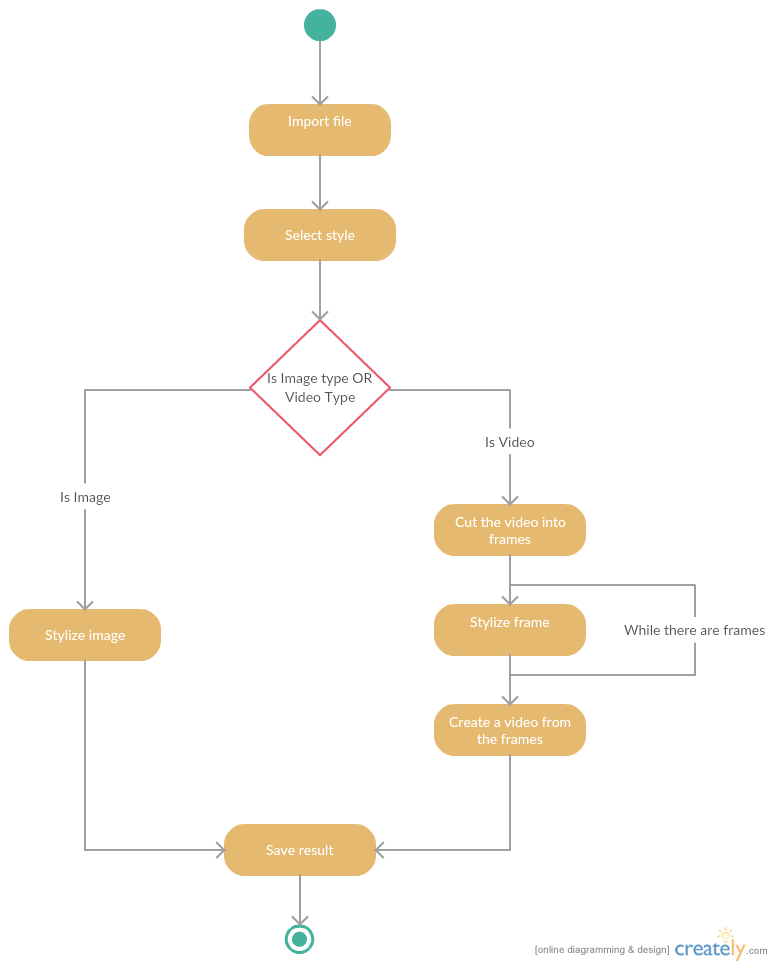
\includegraphics[scale=0.5]{software_overview.png}
		\caption{A rendszer működése felülnézetből}
		\label{felulnezet_1}
	\end{center}
\end{figure}

\section{Párhuzamos gépi tanulás Tensorflow segítségével}
\secro{Învățare automată cu ajutorul librăriei Tensorflow}
\secen{Parallel machine learning using Tensorflow}

\subsection{A Tensorflow alap konceptusai}
\ssecro{Conceptele de bază a librăriei Tensorflow}
\ssecen{The basic concepts of Tensorflow library}

A Tensorflow egy gépi tanításra alkalmas könyvtár. Tensorflow segítségével leírt algoritmus nagyon kevés kódmódosítással számos eszközön futtatható, kezdve a mobil eszközöktől egészen a GPU-kal ellátott osztott rendszerekig. Főleg a deep learning típusú algoritmusok implementálására használatos, viszont flexibilitásából adódóan számos más tanítási folyamat elvégzésére is képes \cite{35}.
\newline
\indent
A Tensorflow működése leírható egy irányított gráf segítségével. A gráf az adat áramlását reprezentálja, míg a gráfban levő csúcsok jelentik a kontrollt az adat áramlása fölött. Egy ilyen gráfban minden csúcsnak 0 vagy több bemenetele van, valamint 0 vagy több kimenettel rendelkezik. Minden csúcs egy operációt jelent. A csúcsok közt folyó adathalmazokat tenzoroknak nevezzük. Valójában egy tenzor egy N dimenziós tömböt jelent. Speciális élek is létezhetnek a gráfban az adatfolyam kontrollálására. Ilyen lehet például egy olyan él, ami megtiltja, hogy adat folyjon át rajta \cite{35}.

\begin{figure}[!htbp]
	\begin{center}
		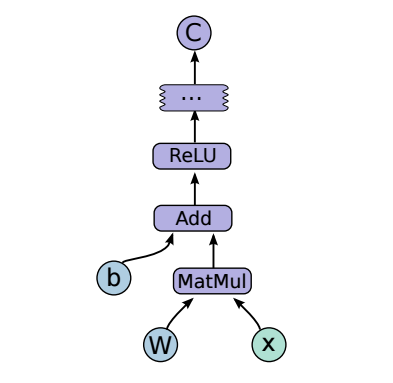
\includegraphics[scale=0.8]{tensorflow_graph.png}
		\caption{Tensorflow számítási gráf\cite{35}}
		\label{tensorflow_graph}
	\end{center}
\end{figure}

Az operációknak lehetnek nevük és attribútumaik. A kernel egy operáció implementációja, ami egy adott típusú hardveren (CPU vagy GPU) fut. Különféle típusú kerneleket különböztetünk meg, amik lehetnek alap matematikai műveletek (összeadás, kivonás, szorzás, osztás, logaritmus, kisebb, nagyobb, egyenlőség, stb.), tömb műveletek (konkatenálás, felvágás, rang, stb.), mátrix műveletek (mátrix szorzás, inverz, determináns, stb.), neuron háló réteg típusok (softmax, szigmoid, ReLu, konvolúciós, stb.), szinkronizációs műveletek (mutex műveletek, sorba állítás) és adatfolyam kontrollálásra szolgáló műveletek.
\newline
\indent
Ahhoz, hogy a számítási gráfban definiált műveleteket elvégezhessük, szessziókat (session) kell definiálni. Szessziók használata megengedi a teljes gráf kiértékelését vagy akár részleges kiértékelést is. A gráf kiértékelése a szesszió Run függvényével történik. 
\newline
\indent
A változó egy olyan tenzor ami megtartja az értékét többszörös számítási gráf kiértékelés esetén is. A változó egy olyan tenzorra utal aminek tartalma megváltozhat, ezzel ellentétben létezik a konstans aminek tartalma nem változhat.
\newline
\indent
A Tensorflow párhuzamosításra úgynevezett processzeket használ (\ref{single_proc_vs_multiple_proc}. ábra). A kliens szoftver egy szesszió interfészen keresztül kommunikál a "master" processzel és a "worker" proceszekkel. Mindenik procesz felelős egy vagy több számítási eszközért (computation device), amik lehetnek CPU magok vagy GPU kártyák. Ezek az eszközök lehetnek lokálisak, ami azt jelenti, hogy ugyanabban a rendszerben helyezkednek el, vagy lehetnek osztottak, ez esetben külön rendszerekben helyezkednek el a különféle eszközök. Minden eszköz saját névvel rendelkezik\cite{35}.

\subsection{Futtatás egyetlen készülék esetében}
\ssecro{Execuție pe un simplu device}
\ssecen{Execution in case of a single device}
Egyetlen eszköz jelenlétében a csúcsok egymást követően lesznek kiértékelve figyelembe véve a közöttük levő dependenciákat. Minden csúcs esetében számolva van, hogy hány dependenciát tartalmaz. Ha ezek közül egyik ki volt értékelve, akkor ez a számláló csökken. Mikor a számláló elérta a 0-át, akkor tovább lép és kiértékeli e következő csúcsot. A kiértékelésre várakozó csúcsok egy listába vannak elhelyezve.

\subsection{Futtatás több készülék esetében}
\ssecro{Execuție pe mai multe device-uri}
\ssecen{Execution in case of multiple devices}
Több készülék esetében szükséges eldönteni, hogy az adott csúcsok melyik készüléken fognak kiértékelődni, valamint fontos megoldani a készülékek közötti kommunikációt.
\newline
\indent
A csúcsok elhelyezése egy mohó esztimációs módszert követ. Minden csúcs esetében megesztimálható, hogy a bemeneti és kimeneti tenzorok mérete byte-ban. Ugyanakkor megesztimálható a futási idő adott csúcsok esetében. Ezután egy szimuláció fog lefutni ami az összes csúcs esetében kilistázza a használható eszközöket majd kiértékeli a futási időt valamit a kommunikáció idejét az eddigi elhelyezett csúcsokkal. A mohó algoritmus szerint egy csúcs arra az eszközre fog kerülni, ami a szimuláció során a legjobb eredményt adta.
\newline
\indent
Az eszközök közötti kommunikációt Send-Receive csúcsok beiktatásával oldja meg. Ezek a csúcsok ugyanakkor megoldják az eszközök közötti szinkronizációt is. Osztott rendszerek esetében ugyancsak Send-Receive csúcsok oldják meg a kommunikációt. Ezek TCP és RDMA protokollokat használnak az adat mozgatásához\cite{35}.

\begin{figure}[!htbp]
	\begin{center}
		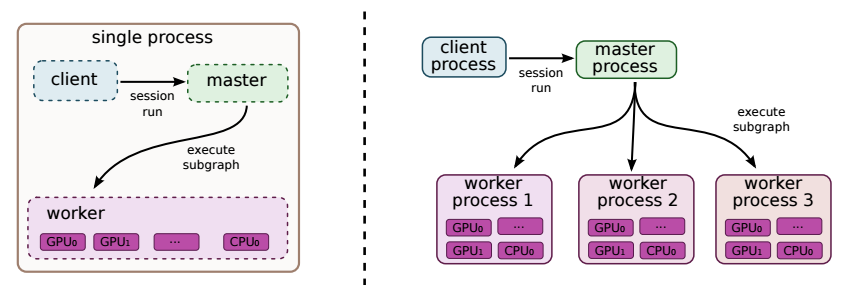
\includegraphics[scale=0.6]{single_proc_vs_multiple_proc.png}
		\caption{Egyetlen procesz összehasonlítása több proceszes működéssel\cite{35}}
		\label{single_proc_vs_multiple_proc}
	\end{center}
\end{figure}

\subsection{Párhuzamos tanítás}
\ssecro{Antrenare paralelă}
\ssecen{Parallel trainig}

A Tensorflow könyvtár a párhuzamosítást megközelíti úgy adatpárhuzamosítás szempontjából, mint feladatpárhuzamosítás szempontjából. Adatpárhuzamosítás esetében az adatot kisebb csomagokba bontja, majd ezeket párhuzamosan bemenetként táplálja a megfelelő csomópontonknak. A kiértékelendő csomópontokból egy másolat kerül az összes szálra (\ref{data_parallel_tf_model}. ábra). A végeredményt egy redukciós művelet gyűjti össze.

\begin{figure}[!htbp]
	\begin{center}
		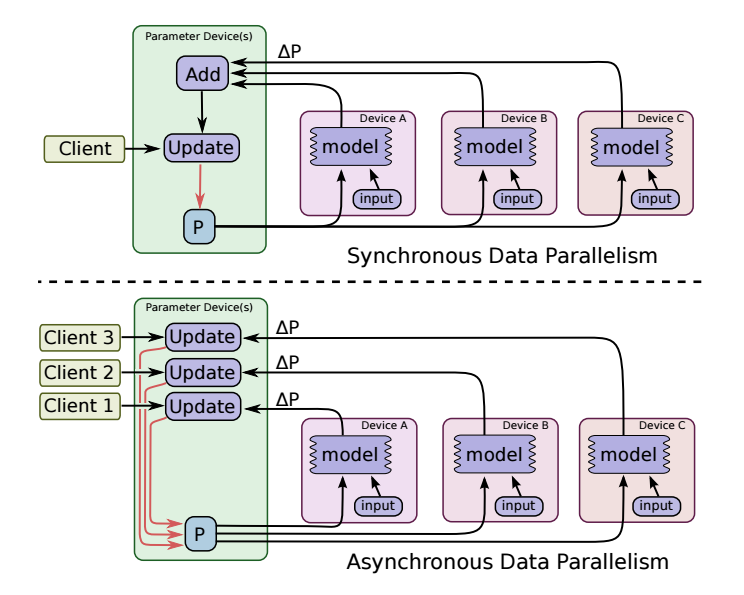
\includegraphics[scale=0.5]{data_parallel_tf_model.png}
		\caption{Adatpárhuzamos szinkron és aszinkron csomópont kiértékelés\cite{35}}
		\label{data_parallel_tf_model}
	\end{center}
\end{figure}

Feladatpárhuzamosítás esetében különböző gráfrészletek lesznek megtanítva ugyanabban az időben különböző szálakon. Mikor a tanítás befejeződik, akkor az a processz egy újabb gráfrészlet kiértékelésének fog neki. Ilyenfajta tanítás esetében fontos figyelembe venni azt, hogy egyes gráfrészletek csak akkor értékelhetőek ki, ha már előttük egy másik gráfrészlet le volt futtatva. Feladatpárhuzamos tanítást a \ref{data_parallel_tf_model}. ábra szemlélteti.

\begin{figure}[!htbp]
	\begin{center}
		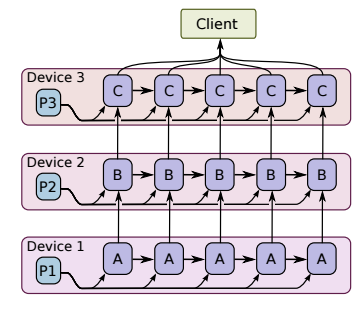
\includegraphics[scale=0.8]{task_parallel_tf_model.png}
		\caption{Feladatpárhuzamos tanítás\cite{35}}
		\label{task_parallel_tf_model}
	\end{center}
\end{figure}


\section{A tanítási módszer állóképek esetében}
\secro{Metoda de antrenare în cazul imaginilor statice}
\secen{Learning method in case of static image inputs}

A rendszer tanításához állokép esetében két bemeneti kép szükséges, az eredeti kép, amire át szeretnénk ruházni a stílust és a stílust tartalmazó kép, aminek a stílusát át szeretnénk ruházni. Mindkét bemenet esetében felírunk egy veszteség függvényt, amik részei a végső nagy tanítási függvénynek.

\subsection{Az eredeti kép tanításának a veszteségi függvénye}
\ssecro{Funcția de pierdere în cazul imaginii originale}
\ssecen{The loss function of the content image}

A mély neurális hálók (Deep Neural Networks) azon típusai amik a legeredményesebbek a képfeldolgozási feladatok elvégzésben a konvolúciós hálók. Mesterséges intelligencia területén a konvolúciós hálók olyan feed-forward típusú neuronhálók, amiket a biológiai elsődleges látókéregről mintáztak. A háló kifejezetten arra volt tervezve és kifejlesztve, hogy kétdimenziós formákat ismerjen fel. A háló alapértelmezetten több rétegből tevődik össze:

\begin{itemize}
	\item konvolúciós réteg: a konvolúciós hálók alapkövei. A réteg súlyai úgynevezett konvolúciós szűrők alkotják, amelyek a forward pass lépés során tanítva vannak. Ez a tanítási lépés úgy történik, hogy a szűrőt végig toljuk a bemeneten és konvolúciónak nevezett műveletet végzünk. 
	\item pooling layer: arra használatos, hogy a bemeneti adathalmaz méretét leszűkítsük úgy, hogy a halmaz adott értékein valamely matematikai műveletet végzünk (átlagszámolás, maximum számolás, minimum számolás). Erre azért van szükségünk, hogy növeljük a tanulás gyorsaságát, csökkentsük a számítások komplexitását megakadályozva ezzel az "overfitting" bekövetkezését.
	\item fully connected layer: minden bemenet mindem más bemenettel kapcsolatban áll.
\end{itemize}

A konvolúciós hálók súlyzókként konvolúciós szűrőket tartalmaznak. Ezek, objektum felisrmerés tanítása esetében, az adott bemeneti kép különböző tulajdonságait fogják tartalmazni. Annak függvényében, hogy a háló topológiájában egy adott réteg hol helyezkedik el, más tulajdonságokat fognak raktározni a szűrök. Az bemeneti réteghez közel álló alacsony szintű rétegek az adott kép pixelinformációit próbálják megjegyezni ezzel szemben a magasabb szinten levő rétegek szűrői különböző tárgyakat, formákat próbálnak megjegyezni\cite{27}\cite{28}. A hálók által tartalmazott információ vizualizálható azáltal, hogy rekonstruáljuk a bemeneti képet a súlyzók alapján. Alacsony rétegek esetében apró módosításokkal visszanyerhető az eredeti kép míg magasabb rétegek esetében objektumok, formák nyerhetők vissza.

Az eredi kép tanításához egy már előre betanított mély konvolúciós neuronhálót használunk fel. A háló tudományos kontextusban VGG-19 név alatt terjedt el amit Simonyan K. és  Zisserman A. vezetett be publikációjukban\cite{29} ahol még a "model E" nevet viselte. Ez a háló gépi látás és tárgyfelismerés céljából volt bevezetve olyan eredményeket produkálva e téren amik az emberi látással versengenek. Rétegei és topológiájának részletes bemutatása a \cite{29} publikációban történik, valamint a \ref{vgg_19} figurán is látható. Fontos megjegyezni, hogy a háló rétegeiből használva volt a 16 konvolúciós réteg, valamint az 5 pooling réteg, a teljesen összekötött rétegek nem voltak használva.

\begin{figure}[!htbp]
	\begin{center}
		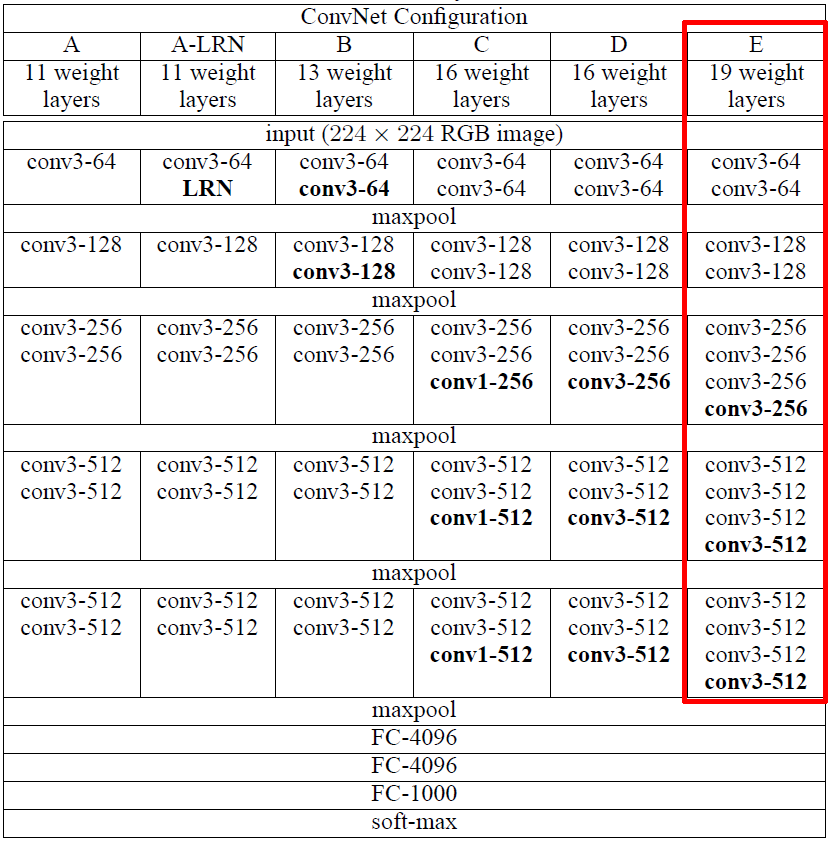
\includegraphics[scale=0.3]{VGG19.png}
		\caption{VGG-19 (Model E) háló topológiája\cite{29}}
		\label{vgg_19}
	\end{center}
\end{figure}

A választás azért esett erre az előre betanított hálóra, mivel Yaroslav N. és Roman N. kutatása alapján\cite{16} összehasonlítva a AlexNet, GoogLeNet VGG-16 és VGG-19 halókat, a VGG-19 használata során sikerült a leglátványosabb képeket készíteni.
\newline
\indent
A konvolúciós neuron háló minden rétege tartalmaz egy adott számú szűrőt, amik különbőző tulajdonságokat tartalmaznak a bementi képről. Ebből kifolyólag maga a bemenet kódolva van a szűrőkben. Egy \(N\) tulajdonságót tartalmazó réteg \(N\) szűrővel rendelkezik, amelyek mérete \(M\). Maga a réteg kimenete lementhető egy \(N * M\) -es mátrixban. Egy adott réteg válasza egy bemeneti képre vizualizálható, ha gradient descent módszert alkalmazunk egy fehér zajt tartalmazó bemeneti képen. Tehát, legyen \(R^l\) egy adott az \(l\) haló válasza egy adott bemeneti képre. Legyen \(W^l\) ugyanaz az \(l\) háló válasza egy adott fehér zajt tartalmazó bemeneti kép esetében. Akkor felírható a veszteségfüggvény mint:

\begin{equation}
L_{content}(\vec{x}, \vec{r}, l) = \frac{1}{2}\sum{R^l_{ij} - W^l_{ij}}
\end{equation}

Ahol \(\vec{x}\) a bemeneti képet jeleni, \(\vec{r}\) pedig azt a kimeneti képet jelenti amit a rendszer generál a rétegek tulajdonságaiból.
Mindez Tensorflow környezetben a következőképpen nézne ki:

\begin{lstlisting}[language=Python]
for layer_name in CONTENT_LAYER:
	content_loss += content_weight * (2 * tf.nn.l2_loss(
		all_layers[layer_name] - content_features[layer_name]) /
		content_features[layer_name].size)

content_loss /= len(CONTENT_LAYER)
return content_loss

\end{lstlisting}

A \(CONTENT\_LAYER\) tuple típusú, ami tartalmazza azoknak a rétegeknek az azonosítóját, amik részt vesznek a veszteség függvény kiszámításában. A mi esetünkben ez egyedül a \(relu4\_2\) kimenetét jelenti, tehát valójában a \(conv4\_2\) konvolúciós réteget használtuk. A \(content\_features\) valtozó egy lista, ez tartalmazza az összes réteg válaszát a bemeneti eredeti képre. A visszaküldött érték egy tensor típusú, egyik részét fogja képezni a végső optimalizálandó veszteségfüggvénynek. 


\subsection{Az stílus kép tanításának a veszteségi függvénye}
\ssecro{Funcția de pierdere în cazul imaginii de stil}
\ssecen{The loss function of the style image}
Az előbbiekben az eredeti bemeneti kép tartalmára voltunk kíváncsiak. A stílus kép esetében viszont nem maga a kép tartalma a fontos. Ebben az esetben egy mintázatot szeretnénk kinyerni a stílusképből. Ehhez fontos megismerni maga a Gram mátrix fogalmát. Hogyha adott egy vektorhalmazunk \(v_1...v_n\), akkor a \(G\) Gram mátrixot a következő eljárás szerint határozzuk meg\cite{30}:

\begin{equation}
G_{ij} = v_i \cdot v_j
\end{equation}

Tehát hogyha az \(A\) mátrixunk oszlopait maga a \(v_1, v_2 ... v_n\) vektorok képezik, akkor a \(G\) Gram mátrix a következőképpen kapható meg:

\begin{equation}
G_{ij} = A A^T
\end{equation}

A Gram mátrix egy szorzatot jelen egy adott vektorhalmaz összes elemei között. A mi esetünkben ez a vektorhalmaz jelentheti egy adott konvolúciós réteg által kiszűrt tulajdonságokat az adott bemeneti stílusképből. Amint már említettem, maga a konvolúciós réteg szűrői egy adott kép tulajdonságait tartalmazzák. A Gram mátrix \(ij\) pozíciójában elhelyezkedő elem megadja, hogy egy adott réteg \(i\)-dik tulajdonsága mennyire teljesül a \(j\)-dik tulajdonság jelenlétében, tehát a két tulajdonság milyen mértékben aktiválódik egyszerre. Ha az \(ij\) pozícion levő elem közelít a \(0\)-hoz, akkor az azt jelenti, hogy a két tulajdonság nem aktiválódik egyszerre, ezzel ellentétben, ha az érték nagy, akkor az azt jelenti, hogy a két tulajdonság nagy valószínűséggel aktiválódik egyszerre.
\newline
\indent
Hogyha az \(l\) rétegnek \(N\) szűrője van, akkor \(G \in R^{N_l*N_l}\), ahol:

\begin{equation}
G^l_{ij} = \sum_{k} F^l_{ik} \cdot F^l_{jk}
\end{equation}

Ahhoz, hogy megkapjuk egy adott háló által generált mintát, textúrát, hasonlóan mint az előzőekben, fehér-zaj képet adunk bemenetként. A veszteségfüggvény egyetlen rétegre felírható mint a fehér-zaj kép Gram mátrixa és a stílus kép Gram mátrixának átlagos négyzetes hibájaként. A \(G\) jelöli a fehér zaj kép Gramm mátrixát, az \(A\) pedig a stílus kép Gramm mátrixát.

\begin{equation}
E_l = \frac{1}{4N^2_l M^2_l} \sum_{i,j} (G_{ij} - A_{lj})^2
\end{equation}

Az összes stílus réteg válasza felírható mint egy összeg, ahol \(w_l\) egy súlyzó faktort jelent:

\begin{equation}
L_{style}(\vec{a}, \vec{x}) = \sum w_lE_l
\end{equation}

A \ref{style_factor}. ábra szemlélteti a stílus súlyzó változtatásának hatását. A bemeneti kép a "Sapientia épülete", a stíluskép Munkácsy Mihály "Vihar a pusztán" mesterműve. Az ábra bemutatja, hogy miképpen változik a kimeneti kép a stílús súlyzójának függvényében.

\begin{figure}[!htbp]
	\begin{center}
		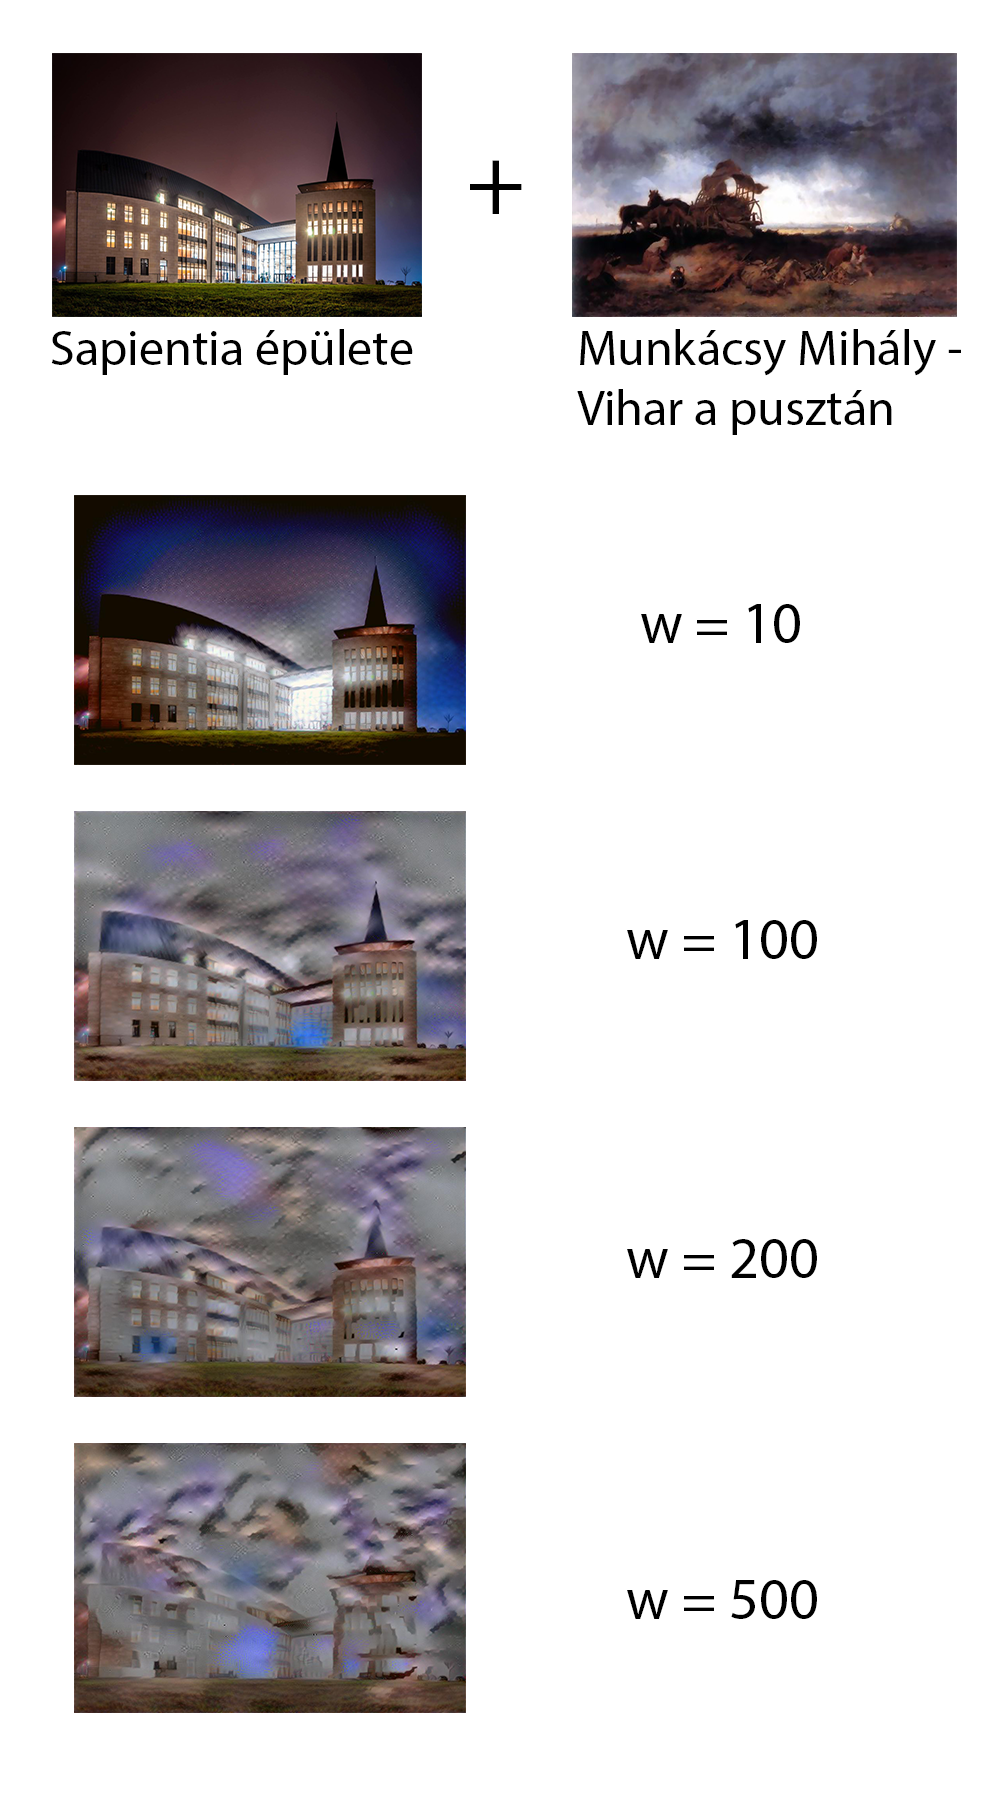
\includegraphics[scale=0.33]{style_factor.png}
		\caption{A stílús súlyzó módosításának eredményei}
		\label{style_factor}
	\end{center}
\end{figure}

A Gramm mátrix számolása Tensorflow környezetben a következőképpen történik:

\begin{lstlisting}[language=Python]
# reshape the tensor to be 2 dimensional
features = tf.reshape(layer, (-1, number_of_channels))
# create Gram matrix which basically is the product of
# the mat with itself
gram = tf.matmul(tf.transpose(features), features) / size
\end{lstlisting}

Maga a veszteségfüggvény meg a következőképpen implementálható Tensorflow könyvtár függvényei felhasználva:

\begin{lstlisting}[language=Python]	
# iterate through style layers
for style_layer in STYLE_LAYERS:
	# get the style layer
	layer = all_layers[style_layer]
	# compute the Gram matrix for the layer
	gram = self._create_gram_matrix(layer)
	# append the gram value to a list
	style_gram = style_features[i][style_layer]
	# compute the style loss for the layer and 
	# add it to a list
	style_loss = style_weight * (2 * 
		tf.nn.l2_loss(gram - style_gram) / style_gram.size)
\end{lstlisting}

A \(style\_features\) valtozó, ugyanúgy mint a \(content\_features\) esetében, egy lista, ez tartalmazza az összes réteg válaszát a bemeneti stílus képre. Az alábbi konvolúciós rétegek kerülnek felhasználásra: \(conv1\_1\), \(conv2\_1\), \(conv3\_1\), \(conv4\_1\), \(conv5\_1\).

\subsection{A stilizált kép tisztítása}
\ssecro{Reducerea zgomotului din imagenea stilizata}
\ssecen{Denoising the stylized image}
A két veszteségfüggvényt alkalmazva sikeresen át tudjuk ruházni a stílust a művészi képről a bemeneti mindennapi képre. Viszont észlelhetjük, hogy az eredmény kép eléggé zajos. Ennek érdekében bevezetünk egy újabb veszteségfüggvényt a zaj csökkentésére, ami a Total Variation Denoising algoritmusra alapszik. Az algoritmus szerint vesszük a stilizált képet és eltoljuk X koordináta mentén egy pixellel, majd az Y koordináta mentén is eltoljuk egy pixellel. Az eltolt képeket kivonjuk az eredi képekből, majd az eredmények abszolút értékeit pixelenként összeadjuk. Ezáltal egy újabb veszteségfüggvényt alítunk elő, amit ugyancsak minimalizálni kell.

\begin{equation}
L_{tv}(\vec{a}, \vec{x}) = \sum_{i,j} \left|(X_{ij} - A_{{i+1}j})\right| + \sum_{i, j} \left|(X_{ij} - A_{i {j+1}})\right|
\end{equation}

Ennek az implementációja pedig:
\begin{lstlisting}[language=Python]	
 tv_loss = tv_weight * 2 * (
(tf.nn.l2_loss(image[:, 1:, :, :] - image[:, :shape[1] - 1, :, :]) /
self.size_of_tensor(image[:, 1:, :, :])) +
(tf.nn.l2_loss(image[:, :, 1:, :] - image[:, :, :shape[2] - 1, :]) /
self.size_of_tensor(image[:, :, 1:, :])))
\end{lstlisting}

\subsection{A teljes veszteségfüggvény felírása és tanítása statikus képek esetében}
\ssecro{Definirea si învățarea funcției de pierdere totala la imagini statice}
\ssecen{The definition and optimization of the total loss function for static images}

Eddig bemutatásra került a stílus kép tanításának veszteségfüggvénye, az eredeti kép veszteségfüggvényének tanítása valamint egy veszteségfüggvény a kimeneti kép zajtalanítására. A végső veszteségfüggvény egyszerűen felírható a három veszteségfüggvény összegeként. 

\begin{equation}
L = L_{content} + L_{style} + L_{tv}
\end{equation}

A teljes veszteségfüggvény tanítására az ADAM\cite{32} optimalizáló algoritmus alkalmaztuk. Az ADAM ( Adaptive Moment Estimation) momentum algoritmus egy sztochasztikus gradiens alapú optimalizáló algoritmus. Az algoritmus felhasználja a elsődleges, valamint a másodlagos gradiensek átlagát ahhoz, hogy a veszteségfüggvényt minimalizálja. Az optimalizálási lépések a következő eljárás szerint történnek:

\begin{equation}
\begin{aligned}
(m_t)_i=\beta_1(m_{t-1})_i + (1 - \beta_1)(\nabla L(W_t))_i \\
(v_t)_i=\beta_2(m_{t-1})_i + (1 - \beta_2)(\nabla L(W_t))^2_i \\
\\
(W_{t+1})_i = (W_t)_i - \alpha \frac{\sqrt{1-(\beta_2)^t_i}}{1-(\beta_1)^t_i} \frac{(m_t)_i}{\sqrt{(v_t)_i} + \varepsilon} \\ 
\cite{33}
\end{aligned}
\end{equation}

\begin{figure}[!htbp]
	\begin{center}
		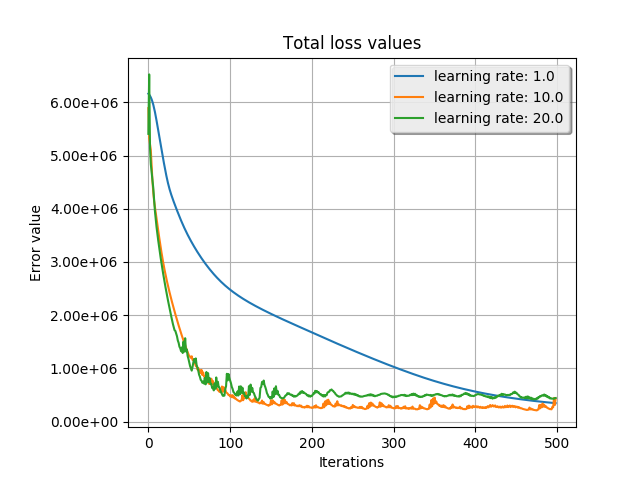
\includegraphics[scale=0.9]{total_loss_values.png}
		\caption{Tanítási függvény optimalizálása különböző tanítási ráták esetében}
		\label{total_loss}
	\end{center}
\end{figure}

Ahol, \(m\) és \(v\) jelentik az elsőfokú valamint másodfokú gradienseket, \(W\) jelenti a súlyzókat, \(\beta_1\) és \(\beta_2\) jelentik a momentumokat, emellet \(\varepsilon\) egy nagyon kis értékű szám annak érdekében, hogy elkerüljük a 0-val való osztást.
\newline
\indent
Értelemszerűen a tensorflow deep learning könyvtár beépítetten tartalmazza a Adam optimalizációs algoritmust, ezért ennek a leprogramozására nincs szükség. 

\section{A tanítási módszer mozgóképek esetében}
\secro{Metoda de antrenare in cazul imaginilor video}
\secen{Learning method in case of video inputs}

\subsection{Naiv megközelítés}
\ssecro{Abordarea naivă}
\ssecen{Naiv approach}

Eddigiekben bemutatásra került miképpen vihető át a stílus egyik statikus képről a másikra. Mindenki tisztába van azzal, hogy egy videó statikus képek sorozatából tevődik össze, amiket képkockáknak (frame) nevezünk. Ennek megfelelően a naiv megközelítés az lenne, hogy ha adott egy videó, akkor vágjuk azt darabokra, pontosabban statikus képkockákra, majd az összes képkockára alkalmazzuk a stílus átruházási módszert.
\newline
\indent
A bemeneti videót frame-ekre való bontásához az ffmpeg nyílt forráskodú alkalmazást használtuk. Az ffmpeg parancssorból futtatható, a következő paraméterek szükségesek, ahhoz, hogy a mozgóképet statikus képek sorozatává alakítsa:

\begin{lstlisting}[language=bash]
ffmpeg -i <input_video_path> -f image2 frame%05d.<ext>
\end{lstlisting}

A \(frame\%05d.<ext>\) egy mintát jelent ami szerint a képkockák elnevezését határozza meg. Az \(<ext>\) a képkockák kiterjesztését jelenti.
\newline
\indent
Miután a stílus átruházása az összes képkockára megtörtént, vesszük az összes stilizált képkockát és felépítjük belölük a kimeneti videót. Ez ugyancsak megoldható az ffmpeg alkalmazással.

\begin{lstlisting}[language=bash]
ffmpeg "-i" frame%05d.<ext> output_name.<ext>
\end{lstlisting}

A naiv megközelítés működik, a kimenet egy olyan videó lesz, amely tartalmazza a bemeneti stíluskép jellegzetességeit. Ugyanakkor észlelhető, hogy az eredmény nem valami esztétikus. Észlelhető, hogy a képkockák közötti átmenet nem folyamatos. Emellett különböző zajokat, úgynevezett "artifact"-eket észlelhetünk. 

\subsection{A haló inicializálása képkockák esetében. Az optical flow bevezetése}
\ssecro{Inițializarea rețelei pentru frame-uri. Introducerea optical flow-ului}
\ssecen{The initialization of the neural net for the frames. Introduction of the optical flow}
Amint említettük, a háló inicalizálására egy fehér-zaj képet használtunk statikus bemeneti képre való stílusátruházáskor. Több képkocka esetében ezzel az a gond, hogy a képkockák nem fognak ugyanabba a lokális minimumba konvergálni tanításkor. Végeredményképp az átmenet egyik képkockáról a másikra nem lesz folyamatos.
\newline
\indent
Egy megoldási kísérlet erre az lenne, hogy ha egy képkocka stilizálása történik, a hálót nem fehér-zaj képpel inicializáljuk, hanem figyelembe vesszük az előtte levő stilizált képkocka és mostani képkocka közötti optical flow-t. Az optical flow egy mozgóképen megjelenő objektum különböző sebességvektorait jelenti. A képet képkocka közötti optical flow megesztimálásával mérhető az adott objektum valós mozgási sebessége. A kamerához távolabb levő objektumok kisebb sebességvektorokkal rendelkeznek, mint azon objektumok amelyek ugyanazon sebességgel mozognak, viszont közelebb vannak a kamerához\cite{34}.
Az optical flow meghatározásához a DeepMatching - Deepflow algoritmust használtuk. Ennek a kimenete egy .flo kiterjesztésű fájl ami tartalmazza adott pixelek esetében a horizontális és vertikális elmozdulás vektorokat. Az optical flow segítségével torzítjuk az előző stilizált képet, ezt az opencv cv2.remap függvényével érjük el. Ez a torzított képpel inicializáljuk a hálót. Ez simább átmenetet fog eredményezni abban az esetben, ha a képkockákon nincs mozgás. Ennek a módszernek a használata szükségszerű viszont nem elégséges ahhoz, hogy szemnek is kellemes eredményt kapjunk.
\newline
\indent
Az optical flow meghatározásával egy mozgóképen meghatározhatók azok a régiók, amik statikusak (adott időn belül az illető régióban nincs változás, úgymond nincs mozgás) valamint azok a régiók ahol új objektumok jelennek meg (olyan objektumok amik eddig esetleg takarva voltak). Fontos nekünk meghatározni azokat a zónákat ahol ilyen objektumok jelennek meg (lásd: \ref{consistency_weights}). Ennek a metódusát Sundaran és társai írják le a \cite{22} publikációjukban.
\newline
\indent
Két egymást követő képkocka esetében meghatározható az optical flow előre, tehát az képkockák időrendi sorrendjében, valamint meghatározható visszafele, az időrendi sorrend ellentett irányában. Jelölje \(w(u, v)\) az előre történő optical flow-t, valamint \(\hat{w}(\hat{u}, \hat{v})\) a visszafele történő optical flow-t. Ekkor felírható az előre történő optical flow torzítása a rá következő képkocka szerint:

\begin{equation}
\tilde{w}(i, j) = w((i, j) + \hat{w}(i, j))
\end{equation}

A mozgás néküli és újonnan megjelenő objektumok nélküli zónák meghatározhatóak a következőképpen:
\begin{equation} \label{eq:1}
|\tilde{w} + \hat{w}|^2 > 0.01(|\tilde{w}|^2 + |\hat{w}|^2) + 0.5
\end{equation}

A mozgási határok pedig meghatározhatóak:
\begin{equation} \label{eq:2}
|\nabla\hat{u}|^2 + |\nabla\hat{v}|^2 > 0.01|\tilde{w}|^2 + 0.002
\end{equation}

A \ref{eq:1} és \ref{eq:2} képletek alapján alkotható egy olyan mátrix, ami tartalmazza a mozgás nélküli zónánkat valamint a mozgási határokat(\ref{consistency_weights}. ábra). Ezt a mátrixot átalakítjuk olyan módon, hogy a mozgási határokra 1-est rakunk, a többi érték 0-ás lesz, jelöljük ez a mátrixot \(c^{(i-1,i)}\)-vel az \(i-1\) és \(i\)-dik képkocka között. Ezt felhasználva felírhatjuk egy újabb veszteség függvényt: 

\begin{equation} \label{eq:2}
	L_{temporal}(x, w, c) = \frac{1}{D}\sum_{k=1}^{D}c_k\cdot(x_k-w_k)^2
\end{equation}

\begin{figure}[!htbp]
	\centering
	\subfloat[Frame00001]{
		
\includegraphics[width=80mm]{input_frame00001.jpg}
	}
	\subfloat[Frame00002]{
		
\includegraphics[width=80mm]{input_frame00002.jpg}
	}
	\hspace{0mm}
	\subfloat[Forward consistency matrix]{
		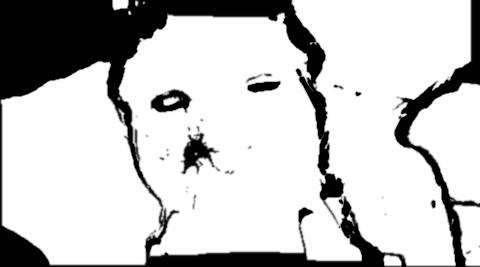
\includegraphics[width=80mm]{forward.jpg}
	}
	\subfloat[Backward consistency matrix]{
		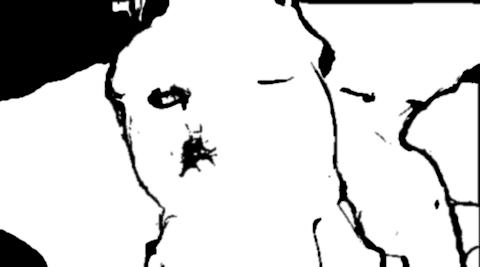
\includegraphics[width=80mm]{backward.jpg}
	}
	\caption{Optical flow két egymást követő képkocka között}
	\label{consistency_weights}
\end{figure}


\section{A rendszer tervezése és kivitelezése}
\secro{Proiectarea și implementarea sistemului}
\secen{The design and implementation of the system}

\subsection{A rendszer interakciós és viselkedési modellje}
\ssecro{Modelul de interacțiune și comportament al sistemului}
\ssecen{Interraction and behavioral model of the system}

A rendszer interakciós modellje (\ref{use_case_diagram}. ábra) a lehető legegyszerűbb. Egyetlen aktort határozunk meg, aki maga a felhasználó. A rendszer esetében nem beszélhetünk bármilyen adminisztrációs felületről mivel nem rendelkezik semmiféle háttértárral valamint pillanatnyilag nem definiál semmiféle hálózati komponenst.
\newline
\indent
A felhasználónak lehetősége van új kép illetve videó anyag bevitelére. Ezt a funkcionalitást egyazon komponens végzi aminek az egyik feladata eldönteni, hogy a kijelölt bemenet kép vagy videó típusú. A felhasználónak lehetősége van a meghatározott kiterjesztésű fájlok közül választani bemenethez.
\newline
\indent
A felhasználónak lehetősége van a rendszer által biztosított stílusok közül választani. A felhasználó nem határozhat meg új stílust. A rendszer nem biztosít erre adminisztrációs felületet.
\newline
\indent
A felhasználó meghatározhatja az átruházási folyamat tanítási paramétereit. A rendszer erre biztosít alapértelmezett értékeket, amiket a felhasználó változtathat. A rendszer megjegyzi az új paramétereket, ezek új indításkor is megmaradnak. A rendszer az alapértelmezett paramétereket is megjegyzi, ezeket a felhasználó bármikor visszaállíthatja az erre kifejlesztett opció használatával.
\newline
\indent
A felhasználó meghatározhatja az útvonalat ahova a kimenet le lesz mentve. A mentést a rendszer automatikusan el fogja végezni az átruházási folyamat után.

\begin{figure}[h]
	\begin{center}
		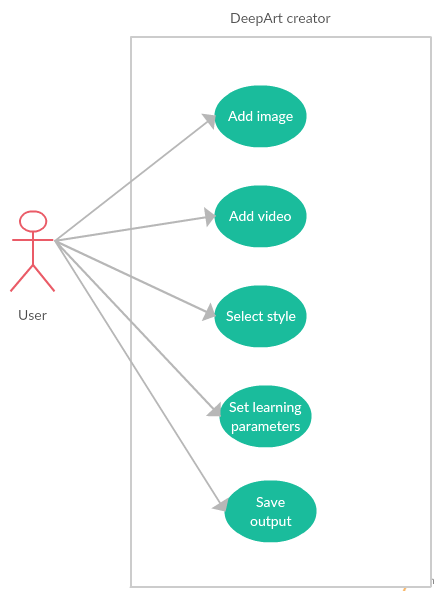
\includegraphics[scale=0.55]{use_case.png}
		\caption{A rendszer viselkedési modellje}
		\label{use_case_diagram}
	\end{center}
\end{figure}

A rendszer interakciós modelljét az \ref{felulnezet_1}. ábra tartalmazza. A felhasználó kiválaszt egy bemeneti állományt a rendszer által meghatározott kiterjesztések közül(.jpg, .png, .gif, .avi, .mp4), majd kiválaszt egy stílust a megadottak közül. A rendszer annak függvényében, hogy milyen bemenetet adtunk, eldönti, hogy kép vagy mozgóképpel kell dolgoznia. Kép esetén lefuttatja a 3.2-es fejezetben ismertetett tanítási algoritmust amely során az átruházza a művészeti kép stílusát. Mozgókép esetén képkockákra bontja azt, majd alkalmazva lesz a 3.3-as fejezet tanítási metódusa. Ha összes képkocka szerkesztve lett, akkor a rendszer felépíti a képkockákból a kimeneti videót. Végezetül a rendszer lementi a megadott helyre a kimeneti állományt.

\subsection{A rendszer strukturális modellje}
\ssecro{Modelul structural al sistemului}
\ssecen{Structural model of the system}

A rendszer a következő komponensekből tevődik össze (\ref{component_diagram}. ábra):
\begin{itemize}
	\item Main Window: az applikáció fő ablaka, ez az ablak jelenik meg az applikáció indításakor, valamint erről az ablakról lehet kiválasztani a bemeneti adatot és a stílus képet. Az ablak Start gombjának a lenyomásával indítható az átruházási folyamat. Az ablak tartalmaz két beágyazott területet, ahol a bemeneti adat, valamint a végeredmény tekinthető meg.
	\item Settings: a főablak menüsorából (Menu Bar) jeleníthető meg. Fő feladata egy grafikus felület biztosítása a különféle beállítások és tanítási paraméterek megadásához. A felhasználó megadhatja az útvonalat ahhoz a mappához, ahova a kimenet lesz tárolva, megadhatja a bemeneti VGG19 háló útvonalat valamint a tanítási paramétereket.
	\item Progress bar: a feladata kimutatni a felhasználó számára, hogy az átruházás milyen státusban van, mennyi van még hátra amig a folyamat befejeződik. Erre azért van szükség, mivel az átruházási folyamat időigényes, ezért fontos a felhasználó tudtára adni, hogy milyen állapotban van a folyamat. A folyamat befejeztekor egy jelzést küld a Main Window komponensnek, ami ki fogja jelezni a felhasználónak a végeredményt.
	\item Artistic Video creator: ez képezi az applikáció magját, ez az a komponens, ami elvégzi maga az átruházási folyamatot. A bemeneti paramétereket/adatokat a Main Window komponenstől kapja. Az átruházási folyamat a videó kártyán fog futni, de ettől függetlenül a komponens jelzéseket fog küldeni a Progress bar komponensnek. Ehhez a komponenshez tartoznak a következő modulok:
	\begin{itemize}
		\item Képkezelő: feladata a bemeneti képek beolvasása és kiíratása a merevlemezre. Beolvasáskor egy preprocesszálás műveletet végez, majd kimenetkor egy posztprocesszálás művelet lesz elvégezve. Fontos megjegyezni, hogy ezt a modult a processzálások miatt nem ajánlott használni a komponensen kívül.  
		\item Videó kezelő: feladata a bemeneti videot képkockákra vágni és a kimeneti képkockákból videót készíteni. A képkockák egy temporális folderbe lesznek elmentve vágás után, ezeknek a beolvasását a képkezelő modul végzi majd.
		\item VGG19 kezelő: a modul feladata ez előre betanított és kimentett VGG19 háló beolvasása és átalakítása egy olyan hálóvá amit a Tensorflow könyvtár fel tud dolgozni majd.
	\end{itemize}
\end{itemize}

\begin{figure}[h]
	\begin{center}
		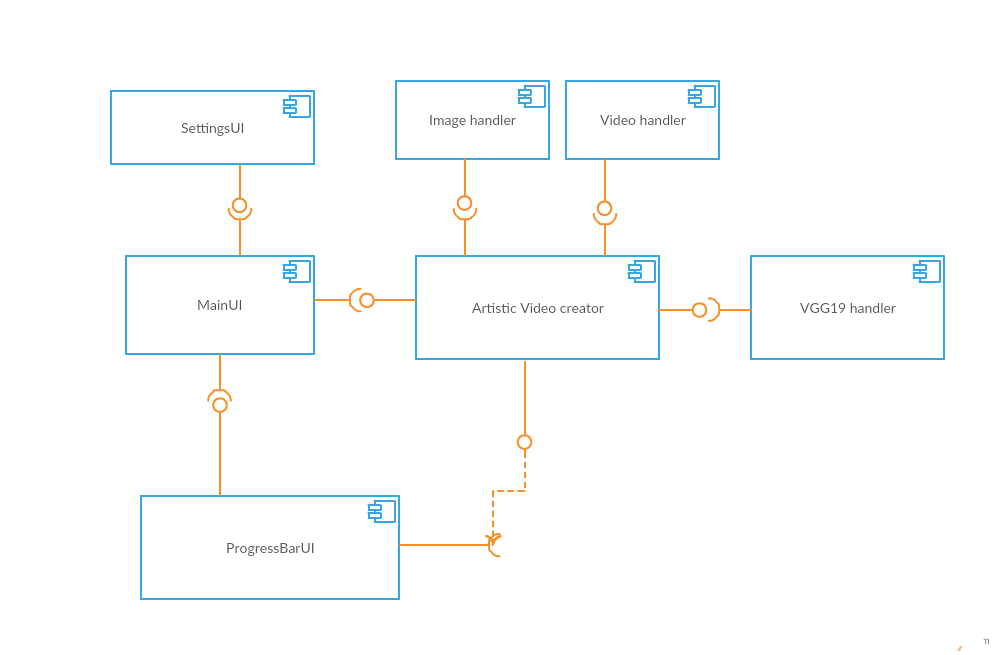
\includegraphics[scale=0.5]{component_diagram.png}
		\caption{A rendszert alkotó komponensek}
		\label{component_diagram}
	\end{center}
\end{figure}

\subsection{Többszálas megoldás és kommunikáció a komponensek között}
\ssecro{Proiectarea pe mai multe fire computaționale a unelor componente}
\ssecen{Multithreaded design and communication of components}

Egy bemeneti képre való stílus átruházás időigényes folyamat. Mozgókép esetében ez a folyamat időigénye lineárisan növekedik a képkockák számának szorzatával. Annak érdekében, hogy az alkalmazásunk reszponzív legyen, elhagyhatatlan aspektus egy olyan modell kialakítása ami igénybe veszi a modern processzorok többszálas működési tulajdonságát. Az "Artistic video creator" komponens működése során ugyan igénybe veszi a videókártya számítási kapacitását, de ez semmiképp sem jelenti azt, hogy a futási idő elhanyagolható. Ugyanakkor fontos kiemelni azt is, hogy azon függvényhívások sorozata ami a videókártyán fognak elvégződni, szinkron módon történnek. Valójában a programunk meghívja az adott függvényt majd addig várakozik, amig megoldás nem érkezett erre.
\newline
\indent
Alkalmazásunk esetében megkülönböztetünk egy főszálat valamint egy mellékszálat (\ref{seq_diagram}. ábra). A főszálon fog futni a Main Window és a köréje csoportosuló felhasználói felülettel rendelkező komponensek, mint például a "Settings" vagy a "ProgressBar". Az alkalmazás indításakor csak a főszál indul el ami létrehozza a "Main Window" és "Settings" komponenseket. Ezt követően, ha a felhasználó megadja a bemeneti állományt, létrejön a "ProgressBar" komponens. A "ProgressBar" azért jön létre csak ebben a pillanatban, mivel a rendszernek tudnia kell a bemenet típusát és ennek függvényében egy factory modell segítségével dönti el, hogy milyen típusú komponens jön létre. Ebben a pillanatban azonban a "Progressbar" komponens még nem látható a felhasználó számára.
\newline
\indent
Ha felhasználó úgy dönt, hogy a megfelelő bemenetet választotta ki, elindíthatja az átruházási folyamatot. Ekkor egy külön szál jön létre (Worker thread), ami átveszi a bemeneti adatokat és elkezdi a folyamatot. A terhelés ebben a pillanatban átkerül a másodlagos szálra, ennek eredményeképp a főszál nem fog blokkolódni. Így az felhasználói felület aktív marad a felhasználó számára és ki fogja tudni szolgálni annak kéréseit.
A munkafolyamat közben az "Artistic Video creator" komponens kapcsolatban áll a "ProgressBar" komponenssel és jelzéseket küld a munkafolyamat státusáról így ez ki tudja jelezni, hogy mennyi munka van még hátra. A munkafolyamat bármikor leállítható még azelőtt, hogy az átruházás befejeződött volna. Ilyenkor a "ProgressBar" üzenetet küld az "Artistic Video creator" komponensnek, ami beállít egy saját leállításra szánt flag-et. A folyamat két iteráció között állítható le, ha az illető flag be volt állítva. Miután a munkafolyamat sikeresen leállt, egy jelzés fog érkezni a "ProgressBar" komponenshez ami majd nyugtázni fogja azt. Ha a munkafolyamat bevégződött, vagy a felhasználó által megszakításra került, a másodlagos szál el fog halni, az ezáltal igényelt erőforrások pedig fel fognak szabadulni.

\begin{figure}[!htbp]
	\begin{center}
		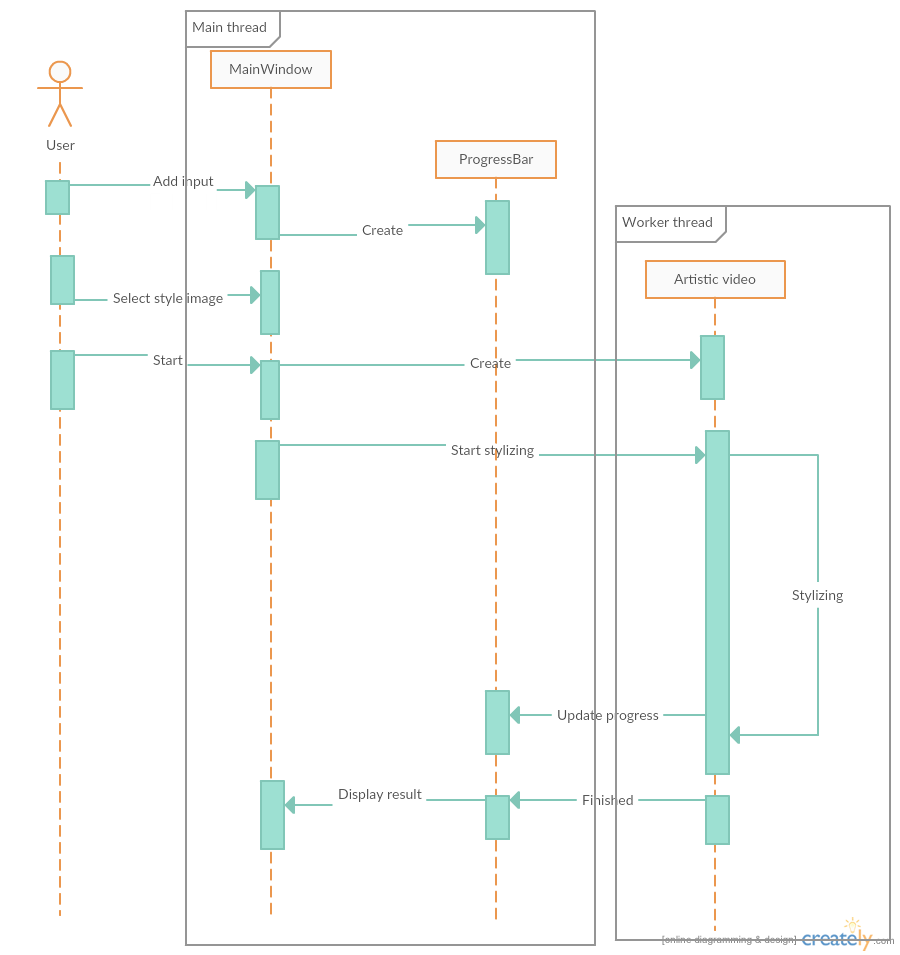
\includegraphics[scale=0.5]{seq_diagram.png}
		\caption{Átruházás szekvencia diagrammja}
		\label{seq_diagram}
	\end{center}
\end{figure}

\subsection{A rendszer implementálása}
\ssecro{Impementarea sistemului}
\ssecen{The implementation of the system}

A rendszer implementációja Python környezetben történt. Ahogy már a bevezetőben is említésre került, az alábbi könyvtárak kerültek felhasználásra: numpy, Tensorflow, opencv, PyQt. Az elkövetkezőkben ki szeretnék térni a PyQt könyvtár bemutatására, ugyanis a szoftver jelentős része ennek a felhasználásával valósult meg és az implementációban használt egyes tervezési minták a PyQt sajátosságait próbálják kiaknázni.
\newline
\indent
A PyQt a híres Qt könyvtárra épül. A Qt egy C++ könyvtár, aminek célja olyan grafikus szoftverek megvalósítása amik különböző platformokat is támogatnak. A Qt univerzális megoldást ad a grafikus felületek elkészítésére, de emellett számos más komponenseket is implementál, mint például tömbök, listák, konténerek, párhuzamos szálak, smartpointerek, hálózati protokollok, stb. A Qt egyik újítása a SIGNAL-ok és a SLOT-ok bevezetése. Ennek működése egyszerű, egy adott osztály adattagjai és metódusai mellett deklarálhatóak SIGNAL-ok és SLOT-ok is. Egy osztály egyes metódusai jelzéseket adhatnak ki SIGNAL-ok segítségével amire a SLOT metódusok csatlakozhatnak. Egy adott SIGNAL kibocsátásakor a rá csatlakozott összes SLOT függvény le fog futni. Például egy grafikus felületen levő gomb lenyomásakor kibocsájtunk egy SIGNAL-t amire a neki megfelelő SLOT függvény meghívódik és lefut. A jelzéskibocsájtás működik többszálas program esetében is, az is megoldható, hogy egy adott jelzésre egy más szálon futó metódus válaszoljon. Természetesen a SIGNAL-SLOT megoldás a PyQt esetében is tökéletesen működik és egy nagyon kényelmes megoldást biztosít a grafikus felület és a business logika összekötésében.
\newline
\indent
A PyQt egy másik előnye az, hogy elegánsan megoldható a modell-nézet-kontroller szoftverfejlesztési minta. Maga a nézet megvalósítható XML leíró nyelv segítségével. Ebből automatikusan generálható egy Python osztály, ami fel fogja építeni maga a kinézetet. Ezt a kontrollerbe be lehet integrálni kompozicióval majd a SIGNAL-SLOT-ok összekötése után használni lehet azt. 
\newline
\indent
A továbbiakban részletes bemutatásra és elemzésre kerül az applikációnk objektum orientált megvalósítása (\ref{class_diagram}. ábra).

\begin{figure}[!htbp]
	\begin{center}
		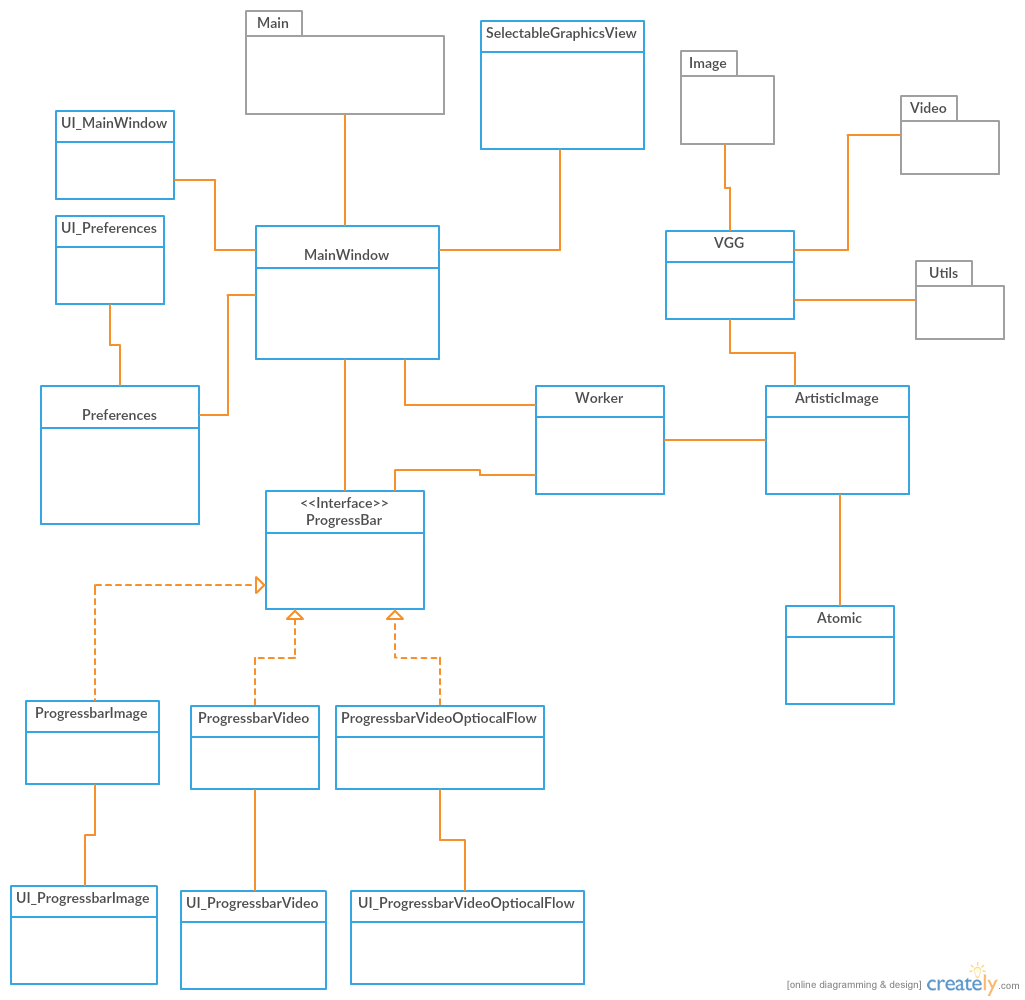
\includegraphics[scale=0.45]{class_diagram.png}
		\caption{A rendszer osztálydiagrammja}
		\label{class_diagram}
	\end{center}
\end{figure}

\subsubsection{A főablak (Main Window) komponens implementálásának bemutatása}
\sssecro{Implementarea componentei Main Window}
\sssecen{The implementation of the Main Window component}

\begin{figure}[!htbp]
	\begin{center}
		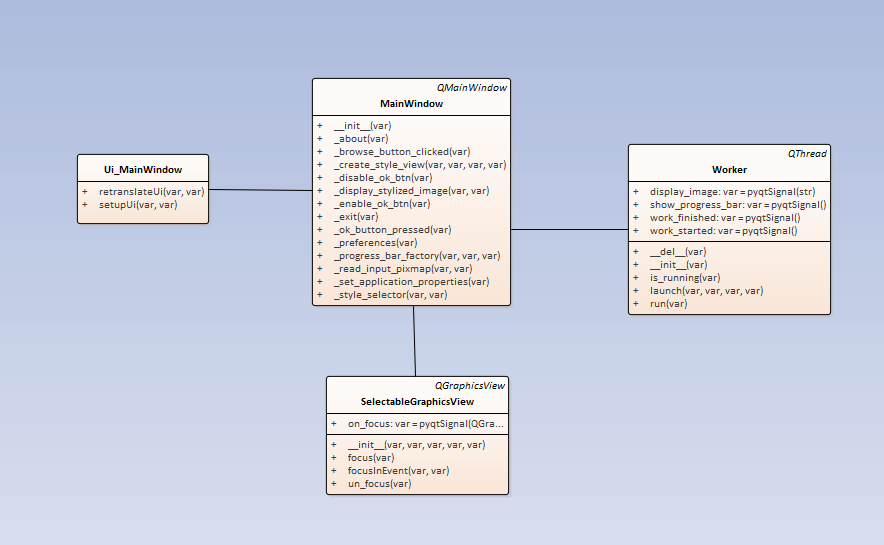
\includegraphics[scale=0.7]{mainwindow_component.png}
		\caption{MainWindow}
		\label{mainwindow_class}
	\end{center}
\end{figure}

A "Main Window" komponens magába foglalja a fő felhasználói implementációját meg pár ehhez szorosan kapcsolódó segítő osztályt(\ref{mainwindow_class}. ábra). Maga a fő ablak megvalósítását két részre bontottuk: maga a nézettel foglalkozó osztály(Ui\_MainWindow) és maga a back-end logikával foglalkozó osztályra (Main Window). Az Ui\_MainWindow egyetlen feladata maga felhasználói felület nézetének definiálása, ezért ezt kompozícióval integráljuk a MainWindow osztályba. A felület (lásd: \ref{graphical_ui)}. ábra) rendelkezik két grafikus kép kijelzésére szánt ablakkal, amik QGraphicsScene típusúak. Ezek közül a bal ablakba fog megjelenni a bemeneti kép amit a felhasználó megad. A QGraphicsScene sajnos nem képes videóanyag beágyazására, ezért az alkalmazás egy előre megadott képet fog ilyenkor kijelezni a felhasználónak. 
\newline
\indent
A bemenet magadása a "Browse..." nyomógomb lenyomásával történik, ami jelzést fog küldeni a \_browse\_button\_clicked metódusnak. Ez létre fog hozni QFileDialog típusú beépített fájlböngésző ablakot. Ez fel van konfigurálva olyan módon, hogy csak az előre kijelölt típusú fájlkiterjesztéseket lehessen beolvasni ("Images/Videos (*.png *.jpg *.gif *.mp4)"). Ha fájlkiválasztás megtörtént, akkor a fájlnak az útvonala megjelenik a "Browse..." nyomógomb melletti szövegdobozban.
\newline
\indent
A MainWindow belső osztályként tartalmazza a SelectableGraphicsView osztályt. Ennek célja a stílusképek közötti váltogatás megoldása(\ref{mainwindow_class}. ábra). Az alkalmazás összes előre definiált stílusképe látható a \ref{styles}. ábrán. Alapértelmezetten a PyQt nem tartalmaz ilyen típusú előredefiniált osztályt, ezért ezt külön le kellett implementálni. A SelectableGraphicsView a QGraphicsView beépített PyQt osztályból származik. Ez azért került választásra mivel a QGraphicsView alkalmas bármiféle statikus grafikus elem beágyazására és ugyanakkor egy olyan területet kínál ami, ha nem fér ki teljesen a képernyőn, akkor scroll-ozni lehet. A SelectableGrahicsView biztosítja, hogy az alkalmazás futásának minden pillanatában egy stílus ki van jelölve. A felhasználó váltogathat ezen stílusok között. A SelectableGraphicsView típusú objektum minden váltogatás esetében jelzést fog küldeni a MainWindow objektumnak, ami lementi azt, hogy az épp kijelölt stílus bemeneti stílus képek a merevlemezen hol található.
\newline
\indent
A főablak egyik fontos objektuma a Worker típusú objektum. Ez a típus a QThread beépített osztály leszármazottja, ami a párhuzamosításért felelős. A Worker típusú objektum felüldefiniálja a QThread run metódusát ami külön szálon fog majd lefutni. Ebben a metódusban lesz létrehozva az ArtisticVideo objektum ami a stílusátruházást végzi. Kezdetben a Worker objektumot a MainWindow inicializálja, az inicializálás még a főszálon történik. Miután ez megtörtént, a főablakon levő "Start" nyomógomb lenyomásával, meghívódik a run metódus. A Worker objektum kapcsolatban áll a MainWindow és a ProgressBar típusú objektumokkal is, amiknek különféle jelzéseket tud küldeni (work\_started, work\_finised, show\_progress, display\_image).
\newline
\indent
Ugyancsak a MainWindow tartalmazza a ProgressBar létrehozásával felelős factory típusú metódust. Amint említettem, a felhasználó "Browse..." lenyomásával beolvashat statikus képet vagy mozgó kép típusú fájlt. Ezekre az átruházás különböző folyamatokat vesznek igénybe. Ahhoz, hogy a felhasználó részletesebb tájékoztatást kapjon arról, hogy mi folyik a háttérben, ezért három típusú progress sávval rendelkező dialógus ablakot implementáltunk le, amik egy közös ősosztállyal rendelkeznek.

\begin{figure}[!htbp]
	\begin{center}
		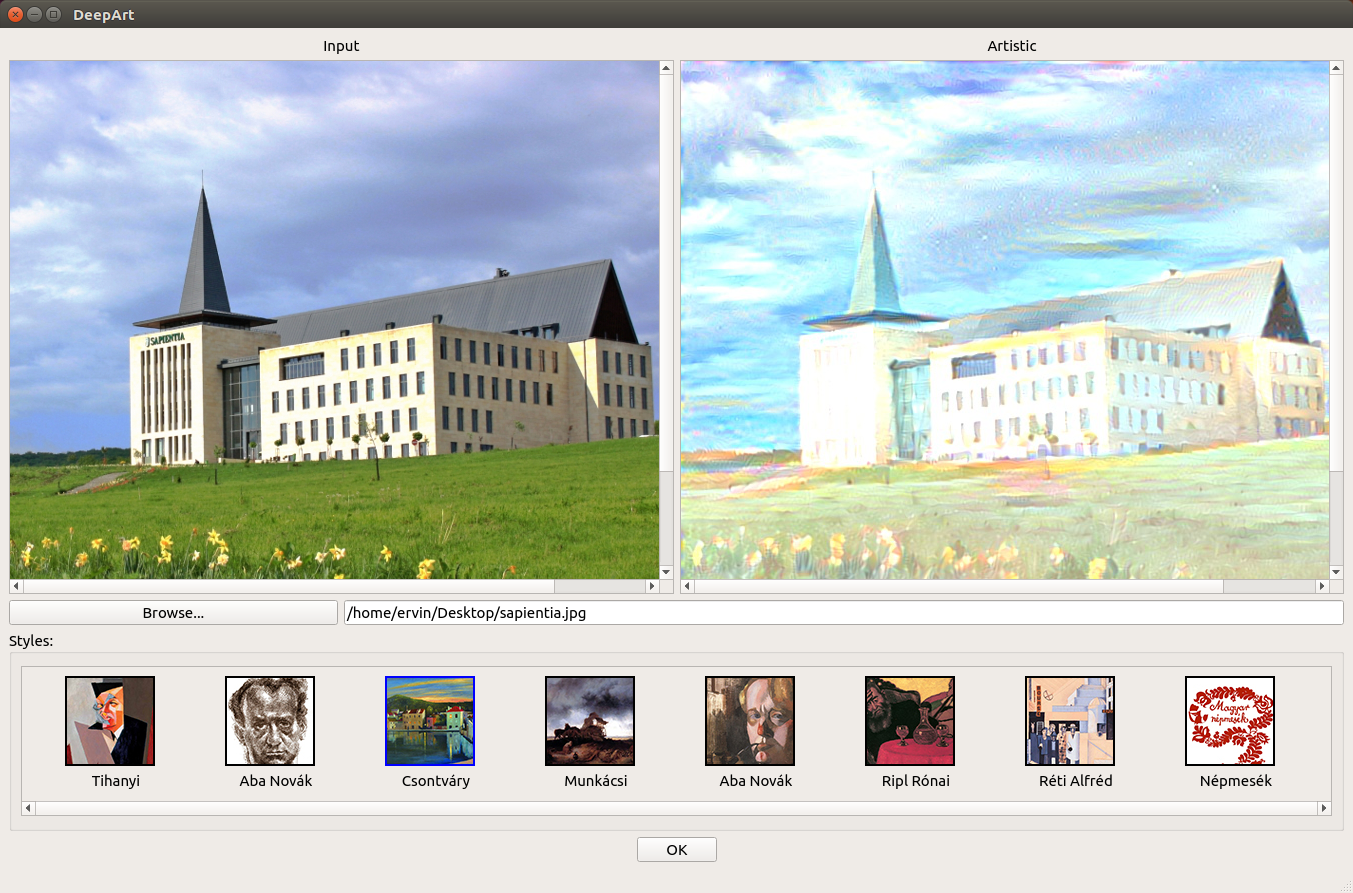
\includegraphics[scale=0.35]{main_ui.png}
		\caption{A rendszer felhasználói felülete}
		\label{graphical_ui)}
	\end{center}
\end{figure}

\begin{figure}[!htbp]
	\centering
	\subfloat[Aba Novak Vilmos - Önarckép]{
		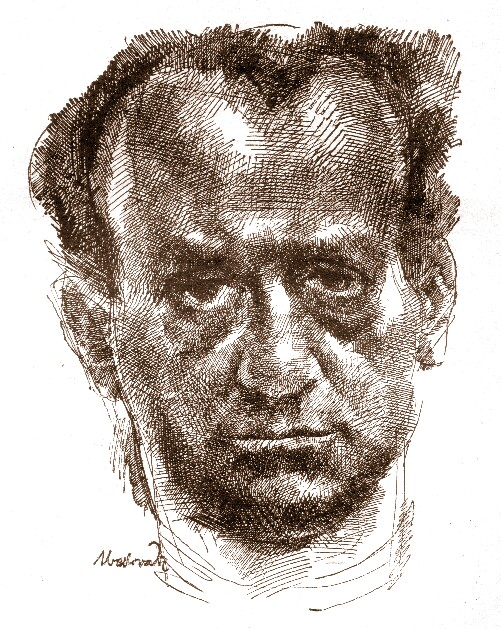
\includegraphics[width=40mm]{stylistic/styles/aba_novak_vilmos_onarckep.jpg}
	}
	\subfloat[Aba Novak Vilmos - Selfportrait]{
		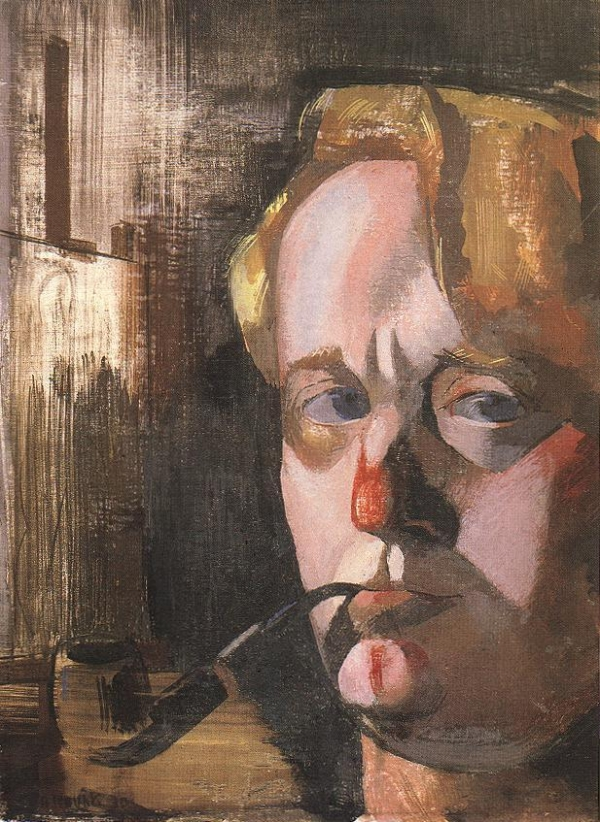
\includegraphics[width=40mm]{stylistic/styles/aba-novak_vilmos_selfportrait.jpg}
	}
	\subfloat[Csontvary Kosztka Tivadar - Traui tájkép naplemente idején]{
		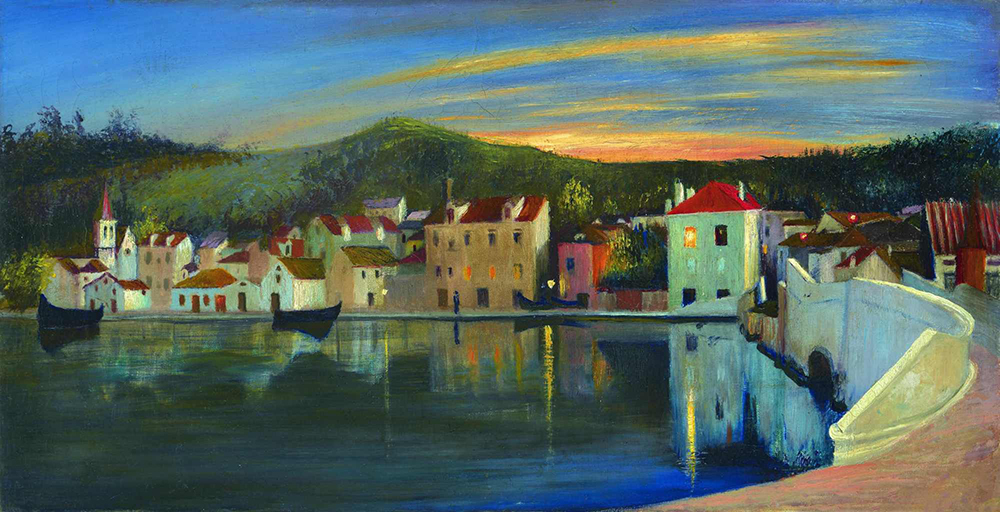
\includegraphics[width=40mm]{stylistic/styles/csontvary_kosztka_tivadar_traui_tajkep_naplemente_idejen.jpg}
	}
	\hspace{0mm}
	\subfloat[Iványi Grunwald Béla - Parkrészlet Kecskeméten]{
		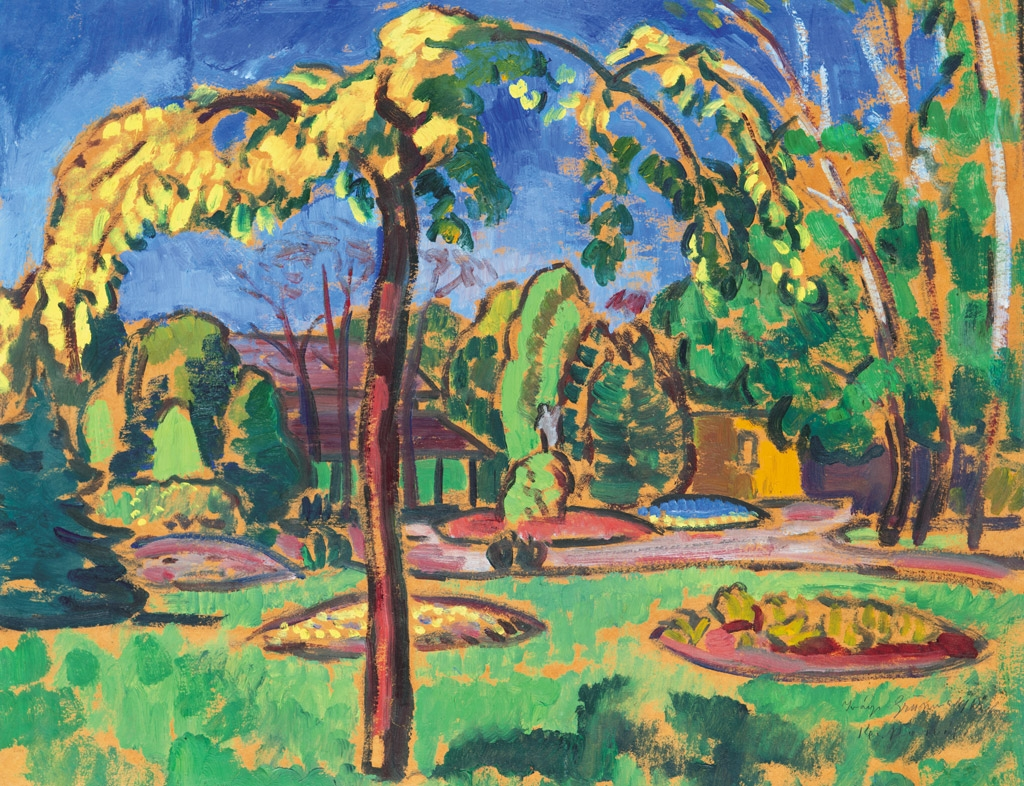
\includegraphics[width=40mm]{stylistic/styles/ivanyi_grunwald_bela_parkreszlet_kecskemeten.jpg}
	}
	\subfloat[Munkácsi Mihály - Vihar a pusztán]{
		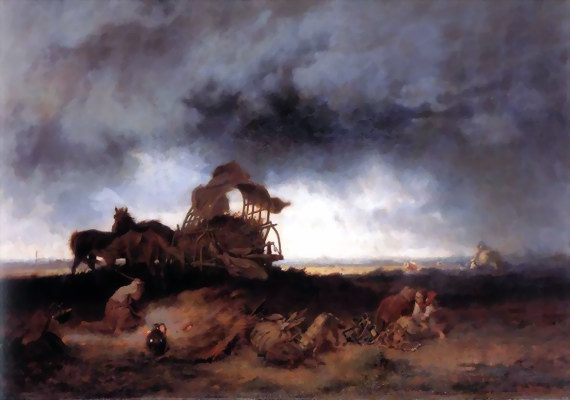
\includegraphics[width=40mm]{stylistic/styles/munkacsi_mihaly_vihar_a_pusztan}
	}
	\subfloat[Réti Alfréd]{
		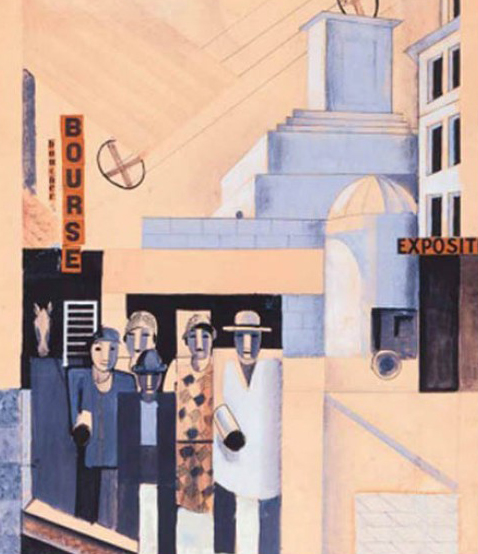
\includegraphics[width=40mm]{stylistic/styles/reti_alfred.jpg}
	}
	\hspace{0mm}
	\subfloat[Ripl-Rónai József - Apám és Piacsek bácsi vörösbor mellett]{
		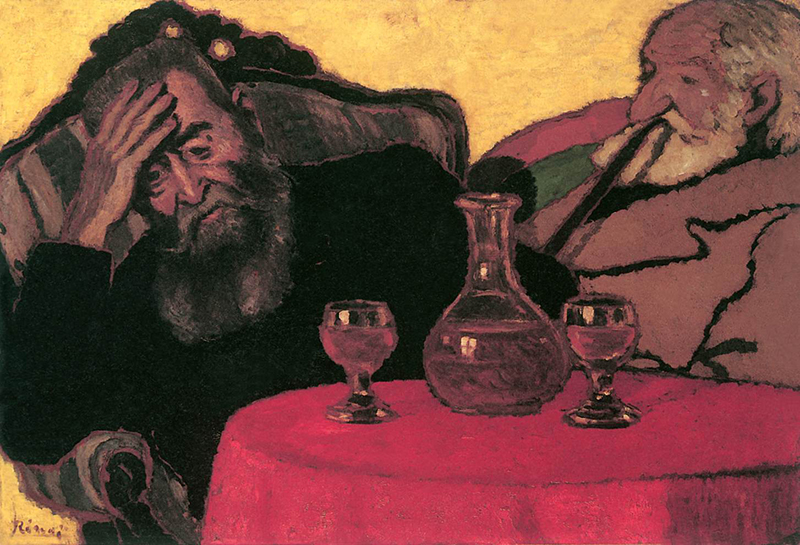
\includegraphics[width=40mm]{stylistic/styles/ripl_ronai_jozsef_apam_es_piacsek_bacsi_vorosbor_mellett.jpg}
	}
	\subfloat[Tihanyi Tzara]{
		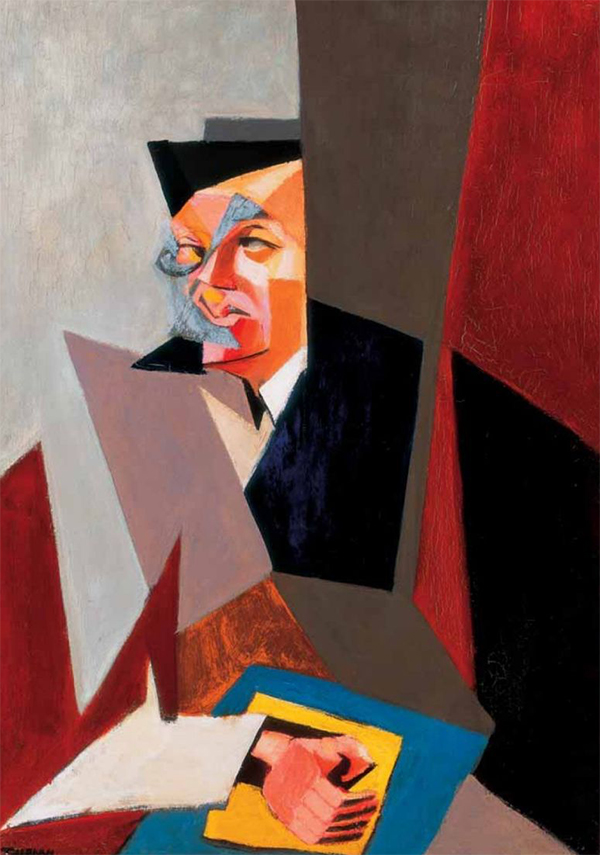
\includegraphics[width=40mm]{stylistic/styles/tihanyi_tzara.jpg}
	}
	\subfloat[Magyar Népmesék]{
		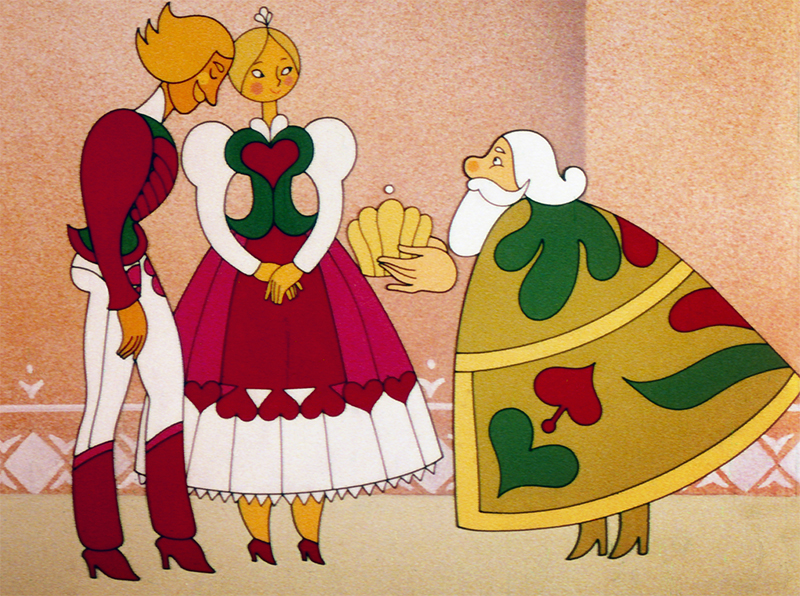
\includegraphics[width=40mm]{stylistic/styles/magyar_nepmesek.jpg}
	}
	\caption{Stílusképek}
	\label{styles}
\end{figure}

\subsubsection{A beállítások (Settings) komponens implementálása}
\sssecro{Implementarea componentei Settings}
\sssecen{The implementation of the Settings component}

\begin{figure}[!htbp]
	\begin{center}
		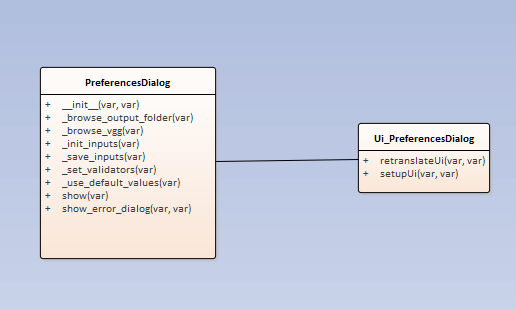
\includegraphics[scale=0.7]{preferences.png}
		\caption{A beállítások komponens osztálydiagrammja}
		\label{preferences_class}
	\end{center}
\end{figure}

A beállítások komponens két objektumot tartalmaz, egyik a PreferencesDialog típusú objektum és az ebbe beágyazott nézetért felelős UiPreferencesDialog objektum. Értelemszerűen a PreferencesDialog tartalmazza a működési logikát.
\newline
\indent
A PreferencesDialog a beépített QDialog osztály leszármazottja, örökli ennek tulajdonságait. Szülő objektumként természetesen a MainWindow objektumot kapja meg, ami Qt-ben annyit jelent, hogy ha a szülő objektum elhal, akkor fel fogja szabadítani a gyerek objektumot is, tehát valójában a szülő objektum felelős a gyerek objektum életciklusáért.
A beállítások dialógus két tab-ot tartalmaz:

\begin{itemize}
	\item Settings: itt meg lehet adni a foldert ahova a kimenet automatikus mentve lesz. Ugyanitt meg kell adni az előre betanított háló útvonalát.
	\item Advanced Settings: itt a tanítással kapcsolatos paramétereket lehet szabályozni. Ilyen paraméterek:
	\begin{itemize}
		\item Learning rate - tanítási együttható 
		\item Iteration per Frame - egy adott képkocka esetében a maximális tanítási iterációk száma;
		\item Content Weight - súlyzó, a bemeneti kép veszteségfüggvénye esetében használatos;
		\item Style Weight - súlyzó, a stílus veszteségfüggvényének az együtthatója;
		\item Temporal Weight - súlyzó, a mozgóképek esetében bevezetett veszteségfüggvény együtthatója.
		\item Use deep flow - egy flag-et állít, ezzel kikapcsolható az időigényes deep flow módszer használata, cserébe gyengébb minőségű videó lesz az eredmény. 
	\end{itemize}
\end{itemize}

Az beállítások komponens tárolja az előre megadott (default) értékeket a paraméterek esetében, ugyanakkor az is el lesz tárolva amit felhasználó módosít ezeken. A módosított értékek megmaradnak akkor is ha az alkalmazást bezárjuk majd újraindítjuk. Erre beépített QSettings objektum használtuk, ami megoldja az beállítások tárolását és visszaolvasását. A QSettings kulcs-érték táblákba tárolja az paramétereket. Ezek majd az applikációnk bármelyik objektumából elérhetőek, ha példányosítjuk a QSettings osztályt és megadjuk az adatbázisunk nevét ahova a paraméterek mentve lettek.
\newline
\indent
Az alapértelmezett beállítások bármikor visszállíthatók a "Use default values" gomb lenyomásával ugyanis ezek a paraméterek hardcode-olva vannak az applikáción belül.

\begin{figure}[!htbp]
	\centering
	\subfloat[Settings tab]{
		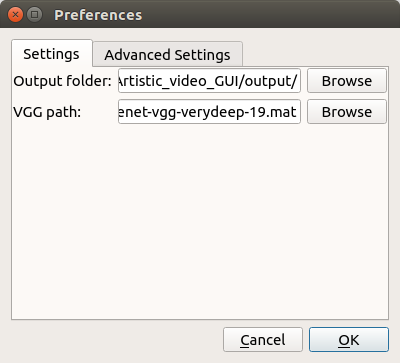
\includegraphics[width=65mm]{settings.png}
	}
	\subfloat[Advanced Settings tab]{
		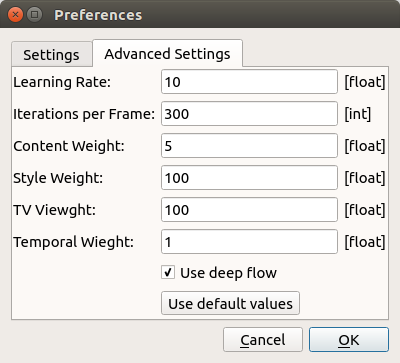
\includegraphics[width=65mm]{advanced_settings.png}
	}
	\caption{Beállítások dialogus ablak}
	\label{settings_dialog}
\end{figure}

\subsubsection{A progress sáv (Progress bar) komponens implementálása}
\sssecro{Implementarea componentei Progress bar}
\sssecen{The implementation of the Progress bar component}

\begin{figure}[!htbp]
	\begin{center}
		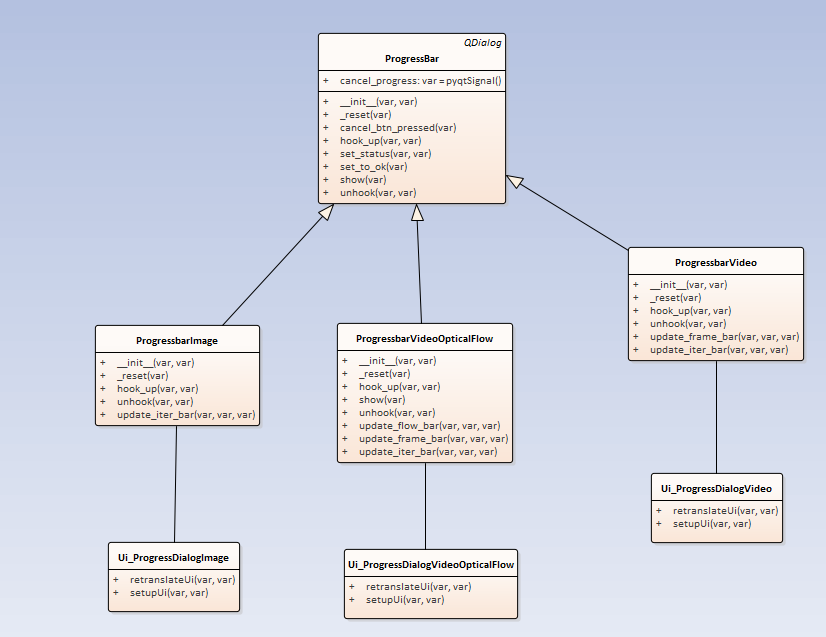
\includegraphics[scale=0.65]{progressbar.png}
		\caption{A progress sáv komponens osztálydiagrammja}
		\label{progressbar_class}
	\end{center}
\end{figure}

A progress sáv komponens feladata kimutatni a felhasználó számára a hátralevő munkamennyiséget. Statikus képek esetében kimutatásre kerül az, hogy az össziterációk számának hány százaléke volt elvégezve. Mozgóképek esetén emellett kimutatásre kerül, hogy a képkockák közül hány százalékre volt stílus átruházva az összes képkockákból. Ha deep flow metódus is használatra kerül, akkor ennek is egy külön sáv fogja valós időben kijelezni, hogy hány képkocka van még hátra, amire alkalmazni kell a deep flow metódust. Ezekből következtethető, hogy három típusú ProgressBar osztály példányosítható, amelyek az alábbiak:

\begin{itemize}
	\item ProgressBarImage(\ref{progressbar_image_ui}. ábra)
	\item ProgressBarVideo(\ref{progressbar_video_no_deeplfow_ui}. ábra)
	\item ProgressBarVideoOpticalFlow (\ref{progressbar_video_deeplfow_ui}. ábra)
\end{itemize}

Mind a három egy közös ősosztályból öröklődik, ez a sima ProgressBar osztály. A ProgressBar osztály a beépített QDialog-ból öröklődik. A QDialog előnye, hogy be meg lehet határozni, hogy amikor a dialógus ablak fókuszban van, akkor ne lehessen interakciónálni a szűlő osztály interfészével. Ez fontos aspektus, mivel amikor maga a stílus átruházás történik, akkor nem szeretnénk, ha a felhasználó a fő ablakkal interakciónáljon, esetlegesen egy másik átruházási folyamatot indítson. Ez az applikáció összeomlásához vezetne.
\newline
\indent
Ahogyan már a MainWindow esetében is bemutatásra került, a ProgressBar típusú osztályok létrehozása a factory modell segítségével történik. Az hogy melyiket fogjuk példányosítani, az a bemeneti állomány típusától, valamint a beállításoktól függ. A ProgressBar ősosztály SLOT metódust tartalmat a "Cancel\textbackslash OK" nyomógomb lekezelésére, és a státus üzenet kiíratására, amit a többi származtatott osztály is örökölni fog. 
A videóval kapcsolatos ablakok emellett SLOT függvényeket definiálnak annak érdekében, hogy ki tudják jelezni hány képkocka van még hátra.

\begin{figure}[!htbp]
	\begin{center}
		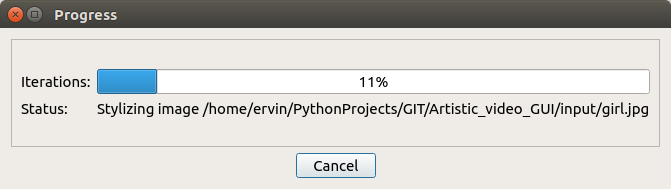
\includegraphics[scale=0.5]{progressbar_image.png}
		\caption{Progress sáv statikus kép esetében}
		\label{progressbar_image_ui}
	\end{center}
\end{figure}

\begin{figure}[!htbp]
	\begin{center}
		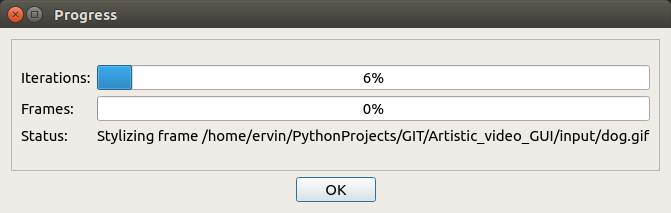
\includegraphics[scale=0.5]{progressbar_video_no_deepflow.png}
		\caption{Progress sáv videó esetében (deepflow kikapcsolva)}
		\label{progressbar_video_no_deeplfow_ui}
	\end{center}
\end{figure}

\begin{figure}[!htbp]
	\begin{center}
		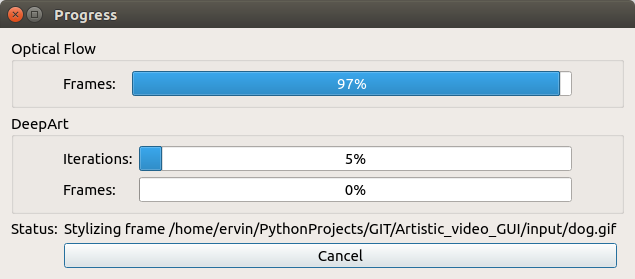
\includegraphics[scale=0.5]{progressbar_video_deepflow.png}
		\caption{Progress sáv videó esetében (deepflow bekapcsolva)}
		\label{progressbar_video_deeplfow_ui}
	\end{center}
\end{figure}

\subsubsection{A stílusátruházó (Artistic video creator) komponens impementálása}
\sssecro{Implementarea componentei Artistic video creator}
\sssecen{The implementation of the Artistic video creatorr component}

\begin{figure}[!htbp]
	\begin{center}
		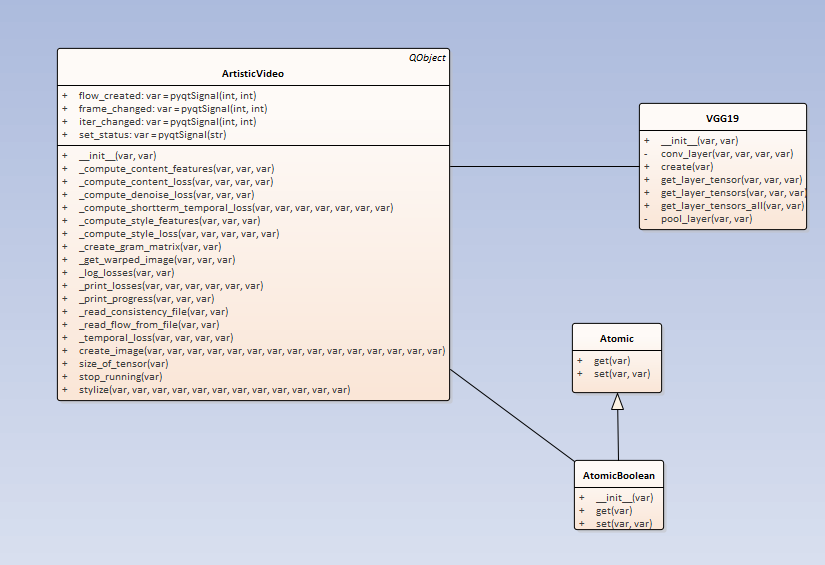
\includegraphics[scale=0.65]{artistic_video.png}
		\caption{A stílusátruházó (Artistic video creator) komponens osztálydiagrammja}
		\label{artisticvideo_class}
	\end{center}
\end{figure}

A stílusátruházó komponenst az ArtisticVideo, VGG19 és AtomicBoolean osztályok alkotják (\ref{artisticvideo_class}. ábra). Ezek körül az ArtisticVideo osztály felelől a stílus átruházásával, a VGG19 osztály felelős az előredefiniált neuronháló beolvasásával. Az AtomicBoolean egy segítő osztály, több szálról is módosítható flag-et definiál. Ezek mellett komponens még használ két csoport segítőfüggvényt amikor az Image meg a Video állományokba csoporosítottuk.
\newline
\indent
Az ArtisticVideo osztályt a Worker objektum példányosítja. Mivel a Worker objektumunk a mellákszálöóon fut, ezzért az ArtisticVideo objektumunk metódusai is a mellékszálon fognak elvégződni. Az ArtisticVideo-nak két fontos metódusa a \(create\_image\) és a \(stylize\). A \(create\_image\) megkapja a bemenet útvonalát, amit az Image vagy Video segítő függvénycsomagok segítségével beolvas és feldolgoz. Amiután ez megtörtént, egyenként minden képkockára meghívódik a \(stylize\) metódus. A \(stylize\) metódus tartalmazza a tanítási algoritmus. Ennek a függvény eredménye minden esetben egy stilizált kép, kivételes eset, ha a tanítás megszakad, ekkor a visszatérített érték a null (\(None\)). Ugyancsak a \(create\_image\) metódusra hárul a képkockákból videót alkotni. 
\newline
\indent
Az ArtisticVideo jelzéseket küld a főablak és a progress dialógus komponenseknek. A Qt kimondja, hogy a felhasználói felület mindenképpen a fő szálon kell fusson ezért az ArtisticVideo nem oldhatja meg az, hogy függvényhívással módosítja a felhasználói felületet. Ez mindenképp jelzéssel kell megoldani, kikötve azt, hogy a jelzésre válaszoló függvény a fő szálon fut. Az ArtisticVideo osztály által definiált jelzések:

\begin{itemize}
	\item flow\_created: akkor bocsájtódik ki amikor egy adott képkocka esetében a deep flow eljárás lefutott. Csak mozgóképek esetében bocsájtódik ki;
	\item frame\_changed: akkor küldődik, amikor egy képkockára sikeresen át lett ruházva a stílus;
	\item iter\_changed: egy kép esetében minden eltelt tanítási iteráció esetén kibocsájtódik;
	\item set\_status: a progress dialógus ablakon levő státus üzenetet lehet állítani ezzel.
\end{itemize}

A VGG19 osztály a bemeneti hálót parszolja és felépíti az alkalmazásban használatos hálót. Mivel a háló mérete nagy (549MB), ezért a merevlemezről történő beolvasás egyszer történik. A háló a memóriában marad amig szükség van erre. Ennek hátránya a memória foglalása, de ekkora memóriahasználat modern számítógépek esetében nem jelent gondot.
\newline
\indent
Ugyanehhez a komponenshez sorolhatunk két segítő (utility) függvényeket tartalmazza csomagot: az egyik csoport az Image, a másik a Video névre hallgat.
\newline
\indent
Az Image csomag tartalmaz egy imread függvényt statikus kép beolvasására és egy imwrite függvényt statikus kép mentésére. Beolvasáskor preprocesszálás történik a bemeneti adaton, ami azt jelenti, hogy a színcsatornákból kivonódnak a következő középértékek: [123.68, 116.779, 103.939]. Ez arra szolgál, a hogy a pixelértékek 0-ás körüli értékeket vegyenek fel. Mentéskör ezek az értékeket hozzáadjuk a kimeneti kép színcsatornáihoz.
\newline
\indent
A Video csomag tartalmaz egy \(convert\_to\_frames\) függvényt ami a megadott útvonalon levő videót képkockákká alakítja. Ezeket a képkockákat majd az imread-del fogjuk feldolgozni. Emellett tartalmazza a \(convert\_to\_video\) függvényt, ami a kimentett képsorozazoz fogja videóvá alakítani. Továbbá tartalmazza a \(make\_opt\_flow\) és \(\_run\_consistency\_check\) függvényeket, amik az optical flow és képkockák mozgási határait eredményezik. Mindkét esetben a függvény egy külső bináris állomány futtatásával végzi el a feladatot. Ezek a binárisok nem saját programkódok a készítők lefordított állományait használtuk fel\cite{34}.

\section{Limitációk}
\secro{Limitații}
\secen{Limitations}
Az implementáláshoz használt Deepmatching és Deepflow algoritmusok esetében a készítők által kiadott binárisokat használtuk. Ezek tökéletesen működnek Linux alapú rendszereken. Mivel a forráskóduk nyílt, ezért megpróbáltuk átírni azokat Windows környezet alá, sajnos többszörös próbálkozás után kénytelenek voltunk feladni. A forráskód eléggé komplex és nem jól dokumentált. Mivel a dolgozat célja nem ez a két algoritmus lefejlesztése köré alapult, ezért inkább abbahagytuk azoknak az átírását. Ennek eredménye az, hogy a Deepmatching és Deepflow által biztosított funkcionalitások nem elérhetőek, ha az alkalmazás Windows operációs rendszer alatt fut.
\newline
\indent
A Deepmatching algoritmus is mesterséges intelligenciát használ, ezért itt is ajánlatos volna VGA megoldást használni. Sajnos a dolgozat elkészítésekor működő megoldás nem volt erre. A VGA-ás megoldás jelentőset gyorsítana az algoritmuson.

%----------------------------------------------------------------
\chapter{A rendszer tesztelése}
\capterro{Testarea sistemului}
\capteren{The testing of the system}

A rendszer tesztelése alatt fel szerettük volna mérni, hogy a ez miképpen viselkedik a mindennapi használatban. Többek között választ szerettünk volna kapni olyan kérdésekre, hogy a rendszer mennyi idő alatt ruházza át a stílust egy statikus képre vagy egy videóra, mekkora a memória igénye, mekkora a maximális képméret amire még működőképes.

\section{A tesztrendszer ismertetése}
\secro{Configurația de test}
\secen{Test configuration}

A rendszer tesztelésére a következő konfigurációt használtuk:

\begin{itemize}
	\item \textbf{Alaplap:} MSI Z170A-G45 GAMING
	\item \textbf{Processzor:} Intel(R) Core(TM) Skylake i7-6700 ("non-K") CPU @ 3.40GHz (Turbo Boost: 3.90GHz)
	\item \textbf{Videokártya:} GIGABYTE GeForce GTX 1080 G1 GAMING 8GB DDR5X 256-bit
	\item \textbf{RAM Memória:} Corsair Vengeance LPX Black 32GB DDR4 3000MHz
	\item \textbf{Merev lemez}: HyperX Savage SSD, 240GB, 2.5", SATA III
	\item \textbf{Operációs rendszer:} Ubuntu 17.04 LTS
\end{itemize}

A használt videókártya egy nVidia GeForce GTX 1080 volt, ennek is a Gigabyte által kiadott G1 GAMING változata. A kártya főleg játékra volt tervezve, de kiemelkedő hardver tulajdonságainak megfelelően tökéletesen használható párhuzamos gépi tanulásra is. A videókártya a Pascal architektúrával rendelkezik. A kártya alapfrekvenciája 1695 MHz, terhelés alatt felugorhat 1860MHz-re. A kártya 2560 CUDA maggal rendelkezik valamint 8GB DDR5X típusú memóriával, amiből gépi tanulásra használható 7860MB.
\newline
\indent 
A rendszer a legújabb Linux Debian alapú Ubuntu operációs rendszeren futott. A rendszer egyes limitációkkal támogatja a Microsoft Windows operációs rendszert is, viszont a limitációk miatt az összes teszt nem végezhető el azalatt, ezért az Ubuntu-ra esett választás. A operációs rendszerünk az ekkori legújabb nVidia driver-ekkel volt ellátva ami a 375.66 verziójú kiadás. A Pascal architektúrát támogató CUDA 8.0-ás videókártya fejlesztő könyvtárat használtuk. Emellett a Tensorflow igényeli a cudnn videó kártya memóriájával foglalkozó könyvtárat is.

\section{Egy képkockára történő stílusátruházási idő és memória igénye}
\secro{Timpul și memoria necesară transferări stilului pe o imagine statică}
\secen{The amount of time and memory needed for transfering the style to a frame}

Első tesztelési esetként az szerettük volna lemérni, hogy mennyi idő szükséges egy statikus képre történő stílusátruházáshoz. A művelethez a videókártya párhuzamos számítási képességeit is igénybe vesszük. Maga a stílusátrhuzás a videókártyán fog történni. Ehhez a teszthez kiválasztottunk pár ismertebb felbontással rendelkező bemeneti képet és mindenik esetben lemértük az átruházáshoz szükséges időd. Az átruházás 300 iteráció alatt történt. Ugyanazt a stílusképet használtunk mindenik bemenet esetében. A stílus kép felbontása $600 \times $855 pixel volt. A következő eredményeket kaptuk (\ref{time_per_res}. 
ábra):

\begin{center}
	\begin{tabular}{ | l | l |}
		\hline
		Felbontás(pixel) & Idő(másodperc) \\ \hline
		$320 \times $240 & 23.126104 \\ \hline
		$640 \times $480 & 82.640347 \\ \hline
		$720 \times $480 & 93.487573 \\ \hline
		$800 \times $600 & 127.973041 \\ \hline
		$1024 \times $764 & 203.892024 \\ \hline
		$1280 \times $720 & 245.769916 \\ \hline
		$1366 \times $768 & 279.945757 \\ \hline
	\end{tabular}
\end{center}

A \ref{time_per_res}. diagrammból lekövetkeztethetjük azt, hogy az igényelt idő lineárisan nő a felbontás növekedésének megfelelően ugyanaz a stílus kép használatával. Az is egyértelművé válik, hogy a stílusátruházás high definition(HD) felbontású képek esetében elég időigényessé válik, ugyanis közel 5 percre van szükség egyetlen bemenet elvégzésére.

\begin{figure}[!htbp]
	\begin{center}
		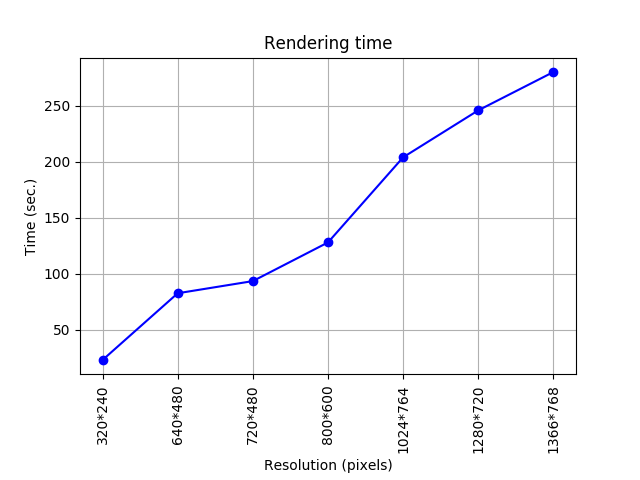
\includegraphics[scale=0.8]{time_per_res.png}
		\caption{Stílusátruházási idő különböző felbontásokra}
		\label{time_per_res}
	\end{center}
\end{figure}

Az előbbi bemeneti képek esetében mérni szerettük volna a videókártya kihasználtságát is. Amint észlelhettük, még az alacsony felbontású képek esetében is eléggé időigényes a folyamat. Feltételeztük, hogy a Tensorflow könyvtár a kártyát maximálisan ki tudja használni. A tesztelési folyamathoz egy teljesen egyedülálló programot készítettünk. Ezt a stílusátruházás előtt el kell indítani. A program a gpustats\cite{36} könyvtárat használja a videókártya működési paramétereinek a lekérdezésére. A programunk minden másodpercben lekéri egyszer a videókártya terheltségi százalékát és kimenti azt egy fájlba amit később fel lehet használni.

\begin{figure}[!htbp]
	\begin{center}
		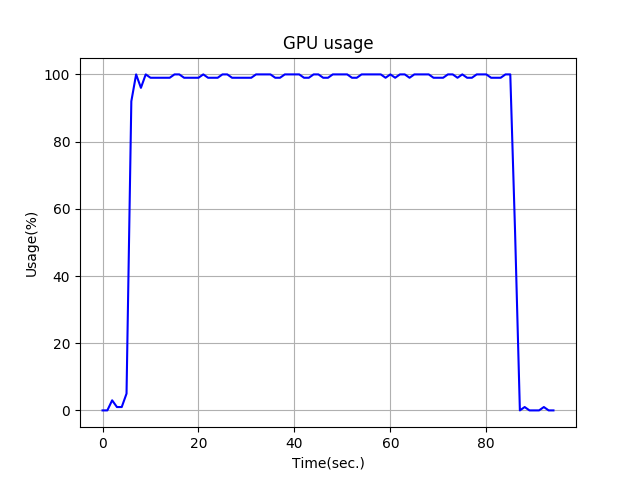
\includegraphics[scale=0.8]{gpu_usage.png}
		\caption{Videókártya terhelése átruházás közben}
		\label{gpu_usage}
	\end{center}
\end{figure}

A \ref{gpu_usage}. diagramm igazolta előrejelzésünket. A videókártya használati százaléka a művelet elején felugrik szinte maximálisra és azon marad addig amig be nem fejezte azt. A \ref{gpu_usage}. ábrán látható diagramm $640 \times $480-as felbontásra keszült, de hasonló eredményeket kapunk bármely más felbontás esetében is.
\newline
\indent
Továbbá azt szerettünk volna mérni, hogy mekkora a memóriahasználat különböző felbontások esetében. Itt a logika azt sugallná, hogy a memóriaigény a felbontásokkal arányosan lineárisan nőni fog. Ezzel ellenben a \ref{gpu_memory_usage}. ábra azt igazolja, hogy a Tensorflow működése nem egyezik meg az előrejelzésünkkel. A memóriahasználatot, hasonlóan mint a kihasználtság esetében, egy külön program méri, ami egy külön processzen fut. A mérésre ugyancsak a gpustats könyvtárat használtuk.

\begin{figure}[!htbp]
	\begin{center}
		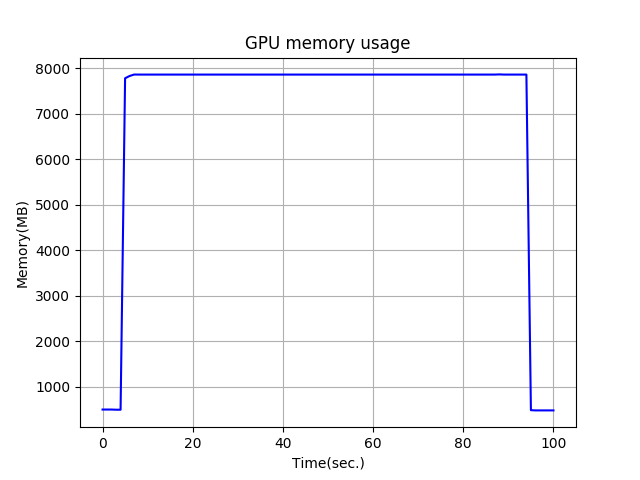
\includegraphics[scale=0.8]{gpu_memory_usage.png}
		\caption{Videókártya memóriájának a kihasználtsága}
		\label{gpu_memory_usage}
	\end{center}
\end{figure} 

A \ref{gpu_memory_usage}. diagramm $640 \times $480 felbontású kép esetében mért értékeket ábrázolja. A videokártyán maximálisan 7860MB volt használható a Tensorflow által. Amint látható, a Tensorflow a kezdetben lefoglalja az összes használható videómemóriát, majd ennek a felhasználásával végzi el a feladatát. A memóriahasználat ugyanakkora $1366 \times $768 felbontás esetében is. Mindez felvet egy másik kérdést, azt hogy mekkora az a maximális felbontás ami még elfér egy GTX 1080 típusú kártya memóriájában?
\newline
\indent
A kérdésre a válasz egyszerűen úgy adható meg, hogy vesszük az ismertebb felbontásokat és próbáljuk addig, amig a Tensorflow nem dob egy memóriával kapcsolatos kivételt. Tovább próbálkoztunk a következő felbontásokkal: $1440 \times $900, $1600 \times $900 és $1920 \times $1080. Ezennel elértük a fullHD minőséget. Statikus kép esetében egy GTX 1080-as kártyával ez meg elfogadható bemenet, viszont itt meg kell említeni, hogy az alkalmazás a HD minőséget célozta. Ebből kifolyólag a stílus képek mérete a HD felbontás környékén mozog. Ez fullHD felbontás esetében bevezethet látható torzulásokat, ami abból adódik, hogy a stílus kép fel lesz skálázva. Tovább haladva $2560 \times $1440 felbontással próbálkoztunk, ami esetében jelentkezett a várt memória kivétel. Tehát a maximális felbontás amit lehetséges használni statikus képes esetében, az a $1920 \times $1080 felbontás.


\section{CPU-GPU futásidő összehasonlítása}
\secro{Compararea timpului necesar pe CPU cu cel necesar pe GPU}
\secen{Comparison of the running timp between CPU and GPU}

Tisztába vagyunnk azzal, hogy a deep learning tanítási módszer alkalmas az adatpárhuzamosításra. Érthető módon elvárt, hogy a processzoron történő futtatás jóval alul kellene maradjon a GPU-un történő futtatással szemben. Ezt igazolják a következő mérések is. Ugyanúgy mint az előző mérések esetében 300 iteráció alatt történt a stílusátruházás. A bemeneti teszt képek is az elöző teszthalmazból vannak kölcsönvéve, ebben az esetben négy felbontásra futtattuk a tesztet. Ez elegendő kellene legyen arra, hogy lássuk a GPU használata által bevezetett gyorsulást. Minden teszt esetben ugyanazt a stílusképet alkalmaztuk, aminek felbontása $600 \times $855 pixel. Az mért eredmények a következők: 

\begin{center}
	\begin{tabular}{ | l | l | l | l| }
		\hline
		Felbontás(pixel) & GPU Idő(másodperc) &  CPU Idő(másodperc) & Gyorsulás\\ \hline
		$320 \times $240 & 23.126104 & 862.980290 & 37.316285\\ \hline
		$640 \times $480 & 82.640347 & 3487.931886 & 42.206162\\ \hline
		$800 \times $600 & 127.973041 & 5446.849902 & 42.562479\\ \hline
		$1024 \times $768 & 203.892024 & 8935.804122 & 43.826158\\ \hline
	\end{tabular}
\end{center}

\begin{figure}[!htbp]
	\begin{center}
		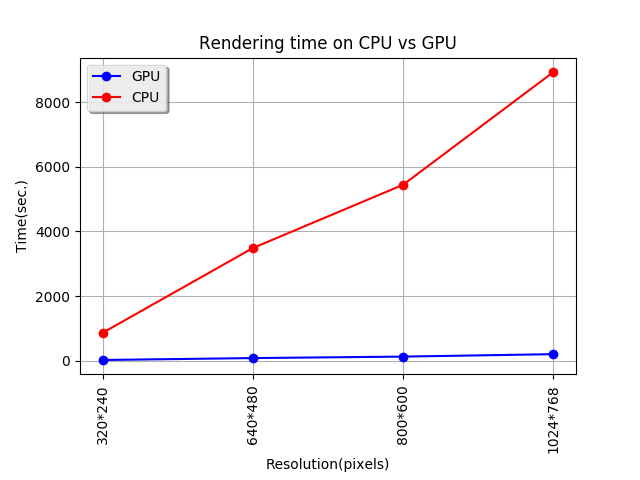
\includegraphics[scale=0.8]{cpu_vs_gpu.png}
		\caption{CPU futásideje összehasonlítva GPU futásidejével}
		\label{cpu_vs_gpu}
	\end{center}
\end{figure}

Előrejelzés szerint a párhuzamosított megoldás sokkal gyorsabb futásidőt igényel. Ahogyan a GPU esetében is láttuk, itt is a felbontás növekedésével lineárisan növekedik a futási idő is. Ami viszont megfigyelhető, hogy alacsonyabb felbontás esetében is a gyorsulás jelentős, $320 \times $240-es felbontás esetében 37-szeres gyorsulásról beszélünk. Ez, ugyan nem ennyire jelentősen, de észlelhetően növekedik a felbontás növekedésével egyaránt (\ref{speedup}. ábra), $1024 \times $768 felbontásnál, közel 44-es gyorsuláról beszélhetünk.

\begin{figure}[!htbp]
	\begin{center}
		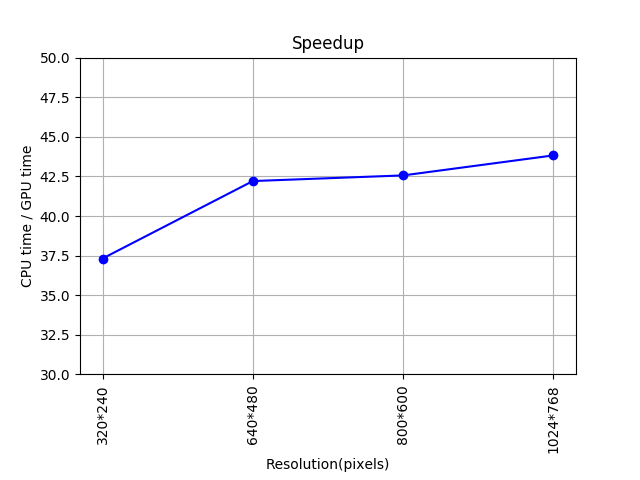
\includegraphics[scale=0.8]{speedup.png}
		\caption{Gyorsulás}
		\label{speedup}
	\end{center}
\end{figure}  

Következtetésképpen kijelenthető, hogy ha rendelkezünk megfelelő videókártyával, akkor mindenképpen azt ajánlott használni. Az előbbiekben bemutatott gyorsulás a CPU és GPU között egyetlen képkockára voltak mérve. Összehasonlításképp, egy $1024 \times $768 felbontású képkocka GPU használatával 300 iterációs átruházás mellett körülbelül 3.4 perc alatt történik, míg CPU használatával körülbelül 149 perc alatt történik. Itt már órás különbségekről beszélünk, tehát mozgókép esetében semmiképp sem ajánlott CPU-t használni. 

\section{Videóra történő stílusátruházás időigénye}
\secro{Timpul necesar transferări stilului pe un videoclip}
\secen{The amount of time needed for transfering the style to a video}

Mindenekelőtt le szerettük volna mérni az optical flow algoritmus futási idejét. Itt megjegyezzük, hogy a programunk a deepmatching - deepflow algoritmust használja. A készítők által szolgáltatott nyílt forrsákodú binárisok lettek integrálva az alkalmazásba. A binárisok a számítógép processzorát használják, hivatalos GPU-ra készített bináris a dolgozat írása idejében nem volt kiadva.

\begin{center}
	\begin{tabular}{ | l | l |}
		\hline
		Felbontás(pixel) & Idő(másodperc) \\ \hline
		$320 \times $240 & 3.700949 \\ \hline
		$640 \times $480 & 71.693549 \\ \hline
		$720 \times $480 & 75.388477 \\ \hline
		$800 \times $600 & 186.4160516 \\ \hline
		$1024 \times $764 & 371.140060 \\ \hline
		$1280 \times $720 & 466.996901 \\ \hline
		$1366 \times $768 & 481.25628 \\ \hline
	\end{tabular}
\end{center}

\begin{figure}[!htbp]
\begin{center}
	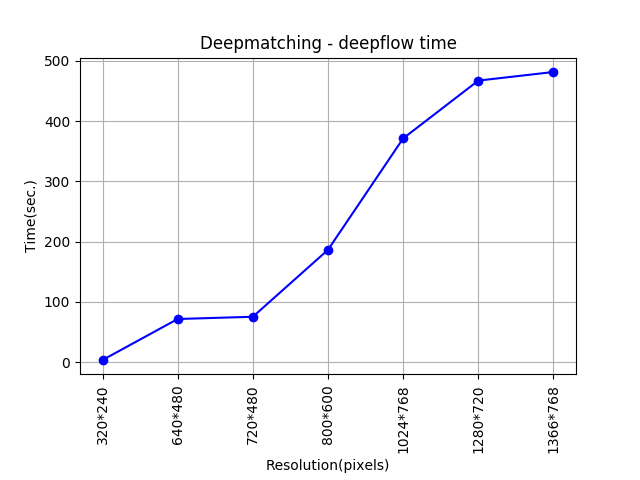
\includegraphics[scale=0.8]{deepmatching_deeplfow.png}
	\caption{Optical flow futási ideje}
	\label{deepmatching_deepflow}
\end{center}
\end{figure}

Az optical flow minden két egymást követő képkocka között ki van számolva mindkét irányba. Ez azt jelenti, hogy ha nekünk például 10 képkockánk van, akkor 9 + 9 flow fájlt kapunk kimenetként. Amint a \ref{deepmatching_deepflow}. diagramm kimutatja, az optical flow eléggé költséges művelet, legtöbb esetben több időbe kerül, mint maga a stílusátvitel. 
\newline
\indent
Továbbá egy 1 perces videóra történő stílusátruházás idejét szeretnénk lemérni. A videó 24 FPS (képkocka/másodperc) paraméterrel rendelkezik, ami azt jelenti, hogy 60 másodperces videó esetében 1440 képkockára kell átruházni a stílust.

\begin{figure}[!htbp]
\begin{center}
	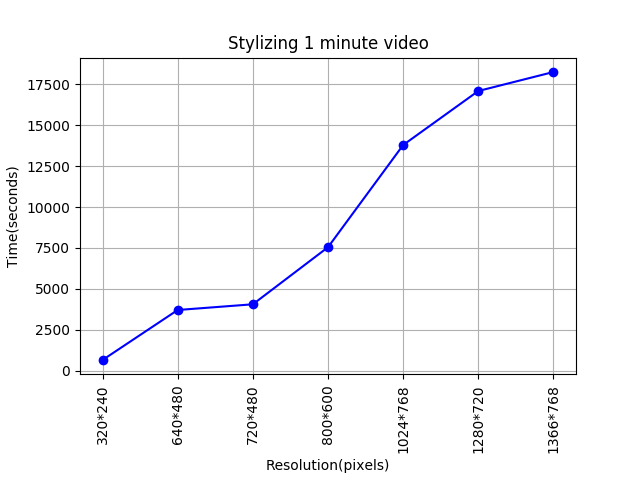
\includegraphics[scale=0.8]{one_min_video_opt_flow.png}
	\caption{Egy perces videóra történő stílusátvitel optical flow használatával}
	\label{one_min_video_opt_flow}
\end{center}
\end{figure} 
 
\begin{figure}[!htbp]
	\begin{center}
		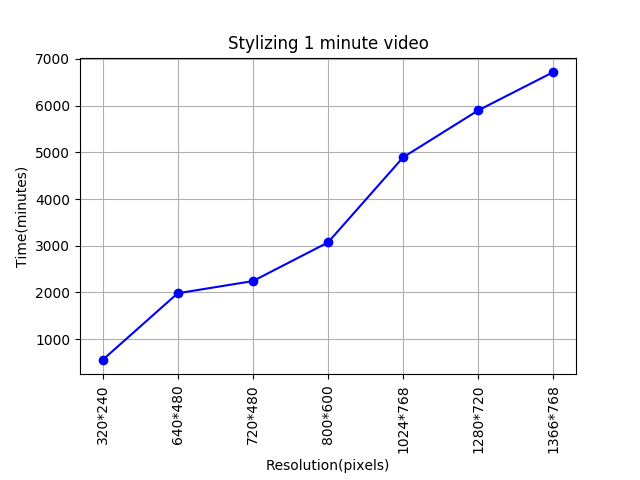
\includegraphics[scale=0.8]{one_min_video.png}
		\caption{Egy perces videóra történő stílusátvitel optical flow használata nélkül}
		\label{one_min_video}
	\end{center}
\end{figure} 

A \ref{one_min_video_opt_flow}. ábrán látható diagramm tartalmazza az optical flow használatával történő átruházást, míg a \ref{one_min_video}. ábrán látható diagramm az optical flow nélküli átruházási időt szemlélteti. Mindkét esetben nagyon időigényes műveletről beszélünk, az első esetében HD felbontás esetében 12 napot futna a program. Ebből azt következtethetjük le, hogy a művelete természetesen kivitelezhető, de annak az időigényével számolni kell. 1 perc videóhoz 12 napos futási idő nem biztos, hogy megéri ez bárkinek a futtatást. Viszont ahogy már láttuk, hardver szempontjábol a Tensorflow nagyon skálázható, ebből a kifolyóla a futási idő simán csökkenthető egy újabb videókártya hozzáadásával. Sajnos erre a dolgozat nem tartalmaz átfogóbb méréseket és tesztelést. 

%----------------------------------------------------------------
\chapter{Összefoglaló}
\capterro{Concluzie}
\capteren{Conclusion}

A dolgozat célja egy olyan rendszer kialakítása és fejlesztése volt, ami képes híres magyar festők festményeinek festészeti stílusát átvenni és átruházni azt olyan képekre valamint videókra, amik nem rendelkeznek különös stílusértékkel. Ehhez egy olyan aztali pc-re szánt alkalmazás kifejlesztése volt a cél, ami képes elvégezni ezt a feladatot. Ezt a célt sikerült is elérni pár limitáció jelenlétében, amiket nem hanyagolhatunk el. 
\newline
\indent
Előszöris sikerült egy olyan applikációt fejleszteni, ami képes statikus képre átruházni egy művészeti stílust. Az applikációt sikerült lefejleszteni Windows valamint Linux alapú rendszerekre úgy, hogy kihasználja a videókártya által biztosított párhuzmosítást. Statikus képre történő stílusátruházás kifogástalanul működik ugyanúgy a Linux valamint Windows rendszereken. Az átruházási idők amint a tesztekből is láthattuk elfogadhatóak abban az esetben, ha rendelekezünk megfelelő videókártyával. Azt is meghatároztuk, hogy noha a rendszer a maximális HD felbontású képek támogatására volt tervezve, működőképes marad akár fullHD felbontású bementi képek esetében is.
\newline
\indent
Továbbá, mozgóképek esetében is próbáltuk megoldani a stílusátruházást. Ez a beépített funkció szintúgy működik Windows valamint Linux rendszerek alatt, megjegyezve azt, hogy Windows alatt nem használható az optical flow algoritmus által bevezetett képminőség javítása. Itt fontos megemlíteni, hogy a dolgozat igazolni tudja, hogy videó esetében is megoldható a stílusátruházás, de ugyanakkor nagyobb felbontások esetében az átruházási idő szempontjából ez nem feltétlenül kifizetödő. Az optical flow metódussal azt próbáltuk elérni, hogy a képkockák közötti átmenet legyen folyamatos elkerülve az úgymond "artifact"-et megjelenését. Ezt sikerült is elérni, viszont a hátránya az, hogy az időigény több mint duplájára növekedett.
\newline
\indent 
Következtetésképpen levonható az, hogy az általunk ismertett megoldások működőképesek, de még szükség van a továbbfejlesztésekre és optimalizációkra ahhoz, hogy egy mindennapi felhasználó által a szoftver gond nélkül használható lehessen.

\section{Továbbfejlesztési lehetőségek}
\secro{Dezvoltare ulterioară}
\secen{Future improvements}

A továbbfejlesztési lehetőségeket három csoportba sorolhatnánk: az álloképre történő stílusátvitellel kapcsolatos fejlesztése lehetőségek, a videóra történő stílusátruházással kapcsolatos fejlesztési lehetőségek valamint maga a szoftver fejlesztésével és működéséval kapcsolatos továbbfejlesztési lehetőségek.
\newline
\indent
A állókép stilizálása esetében a performanciát javítani lehetne azzal, hogy a VGG19 háló helyett egy saját halót betanítunk komondottan erre a célra. Yaroslav Nikulin és Roman Novak tudományos kutatása\cite{16} is ezt javasolja. Ugyanakkor az eredmény kép minőségén is lehetne javítani. Természetesen, a jelenleg fejlesztett program lehetőséget ad a tanítási paraméterek módosítására, viszont ajánlott lenne tovább kisérletezni ezekkel. A tanítás az ADAM tanítási módszert alkalmazza, ezzel szemben tovább lehetne kisérletezni más módszerekkel is esetleges idő és képminőség javítása érdekében.
\newline
\indent
Mozgóképek esetében alapértelmezetten az idő javítása lenne a cél. Ez megoldható lenne többféle módon:
\begin{itemize}
	\item a Deepmatching - Deepflow algoritmus párhuzamosításával és GPU-ra történő leimplementálásával, amint láthattuk jelentős időjavulást lehet eléri adatpárhuzamos feladatok esetében
	\item a Deepmatching - Deeplfow algorirtmus helyett valami más algoritmust használni ami vélhetőleg gyorsabb futási időt eredméynez.
\end{itemize}

Szoftverfejlesztés szempontjából javítani lehet maga a szoftver használhatóságán, kinézetén. Amint már említve volt az optical flow csak Linux alapú rendszereken támogatott, ezt át lehetne írni Windows alapú rendszerekre is. Továbbá fontos lenne egy komolyabb tesztelési mechanizmusnak alávetni az alkalmazást, ugyanis a fejlesztés során ez nem volt feltétlenül szem előtt tartva.
\newline
\indent
A szoftver annak köszönhetően, hogy olyan környezetben íródott, valamint olyan könyvtárakat használ amik multiplatform támogatással rendelkeznek, valószínüleg futna OSX alapú rendszereken is, viszont ilyen alapú kísérlet nem volt végezve a fejlesztés alatt. A továbbiakban erre is ki lehetne térni. 
\newline
\indent
Végezetül pedig, manapság eléggé elterjedtek a cloud alapú szolgáltatások. Azt is javasolt lenne megoldani, hogy az applikációnkból cloud alapú szolgáltatást készítsünk, amit bárki igénybe vehet akár mobilos eszközökről is.


% Ábrajegyzék
%---------------------------------
\newpage
 \listoffigures


% thebibliography
%---------------------------------
\newpage
\begin{thebibliography}{1}

\bibitem {1}
Krizhevsky, A., Sutskever, I., and Hinton, G. E. ImageNet classification with deep convolutional neural networks (2012)

\bibitem{2}
Zeiler, M. D. and Fergus, R. Visualizing and understanding convolutional networks (2013)

\bibitem{3}
\url {https://en.wikipedia.org/wiki/CUDA} (2017.04.24)

\bibitem{4}
\url {http://caffe.berkeleyvision.org} (2017.04.24)

\bibitem{5}
\url {https://keras.io/} (2017.04.24)

\bibitem{6}
\url {http://deeplearning.net/software/theano/} (2017.04.24)

\bibitem{7}
\url {https://www.tensorflow.org/} (2017.04.24)

\bibitem{8}
\url {http://torch.ch/} (2017.04.24)

\bibitem{9}
\url {https://computerstories.net/microsoft-computer-outperforms-human-image-recognition-12028} (2017.04.29)

\bibitem{10}
Kevin Alfianto, Mei-Chen Yeh, Kai-Lung Hua - Artist-based Classification via Deep Learning with Multi-scale Weighted Pooling (2016)

\bibitem{11}
Rosenblatt F. - The Perceptron: A Probabilistic Model For Information Storage And Organization In The Brain (1958)

\bibitem{12}
Werbos, P.J. - Beyond Regression: New Tools for Prediction and Analysis in the Behavioral Sciences (1975)
 
\bibitem{13}
LeCun, Yann, Léon Bottou, Yoshua Bengio, Patrick Haffner - Gradient-based learning applied to document recognition (1998)

\bibitem{14}
Dave Steinkraus, Patrice Simard. Ian Buck - Using GPUs for Machine Learning Algorithms (2005)

\bibitem{15}
Gatys, L. A., Ecker, A. S., Bethge - A neural algorithm of artistic style (2015)

\bibitem{16}
Yaroslav Nikulin, Roman Novak - Exploring the Neural Algorithm of Artistic Style (2016)

\bibitem{17}
Justin Johnson, Alexandre Alahi, Li Fei-Fei - Perceptual Losses for Real-Time Style Transfer and Super-Resolution

\bibitem{18}
Ulyanov, D., Lebedev, V., Vedaldi, A., and Lempitsky - Texture networks: Feed-forward synthesis of textures and stylized images

\bibitem{19}
Ulyanov, D., Lebedev, V., Vedaldi, A., and Lempitsky - Instance Normalization: The Missing Ingredient for Fast Stylization

\bibitem{20}
\url{https://en.wikipedia.org/wiki/Prisma_(app)} (2017.04.29)

\bibitem{21}
Manuel Ruder, Alexey Dosovitskiy, Thomas Brox - Artistic style transfer for videos (2016)

\bibitem{22}
Sundaram, N., Brox, T., Keutzer, K. - Dense point trajectories by gpu-accelerated large displacement optical flow (2010)

\bibitem{23}
\url{https://www.python.org/} (2017.04.30)

\bibitem{24}
\url{http://www.numpy.org/} (2017.04.30)

\bibitem{25}
\url{https://www.riverbankcomputing.com/software/pyqt/intro} (2017.04.30)

\bibitem{26}
\url{http://opencv.org/} (2017.04.30)

\bibitem{27}
Gatys, L. A., Ecker, A. S., Bethge, M. Texture synthesis and the controlled generation of natural stimuli using convolutional neural networks (2015)

\bibitem{28}
\url{https://research.googleblog.com/2015/06/inceptionism-going-deeper-into-neural.html} (2017.05.01)

\bibitem{29}
Simonyan, K., Zisserman, A. - Very Deep Convolutional Networks for Large-Scale ImageRecognition (2015)

\bibitem{30}
\url{http://mathworld.wolfram.com/GramMatrix.html} (2017.05.02)

\bibitem{31}
\url{https://en.wikipedia.org/wiki/Total_variation_denoising} (2017.05.03)

\bibitem{32}
Kingma D. P., Lei Ba, J. - ADAM: A method for stochastic optimization (2015)

\bibitem{33}
\url{http://caffe.berkeleyvision.org/tutorial/solver.html} (2017.05.14)

\bibitem{34}
\url{https://www.mathworks.com/discovery/optical-flow.html} (2017.05.18)

\bibitem{35}
Martin Abadi, Ashish Agarwal, Paul Barham, Eugene Brevdo, Zhifeng Chen, Craig Citro, Greg S. Corrado, Andy Davis, Jeffrey Dean, Matthieu Devin, Sanjay Ghemawat, Ian Goodfellow, Andrew Harp, Geoffrey Irving, Michael Isard, Yangqing Jia, Rafal Jozefowicz, Lukasz Kaiser, Manjunath Kudlur, Josh Levenberg, Dan Mane, Rajat Monga, Sherry Moore, Derek Murray, Chris Olah, Mike Schuster, Jonathon Shlens, Benoit Steiner, Ilya Sutskever, Kunal Talwar, Paul Tucker, Vincent Vanhoucke, Vijay Vasudevan, Fernanda Viegas, Oriol Vinyals, Pete Warden, Martin Wattenberg, Martin Wicke, Yuan Yu, and Xiaoqiang Zheng - TensorFlow: Large-Scale Machine Learning on Heterogeneous Distributed Systems (2015)

\bibitem{36}
gpustats library: \url{https://github.com/dukestats/gpustats} (2017.06.04)


\end{thebibliography}

\newpage
\appendix
\chapter*{Függelékek}
\begin{subappendices}
	\section*{Példák stilizált képekre}
		\begin{figure}[!htbp]
			\begin{center}
				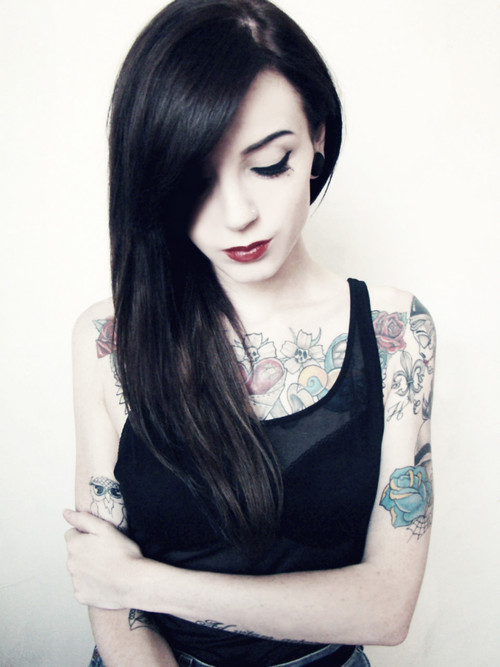
\includegraphics[scale=0.3]{stylistic/original/girl.jpg}
				\caption[]{Eredeti kép}
				\label{original_girl}
			\end{center}
		\end{figure} 
		
		\begin{figure}[!htbp]
			\centering
			\subfloat[Stíluskép]{
				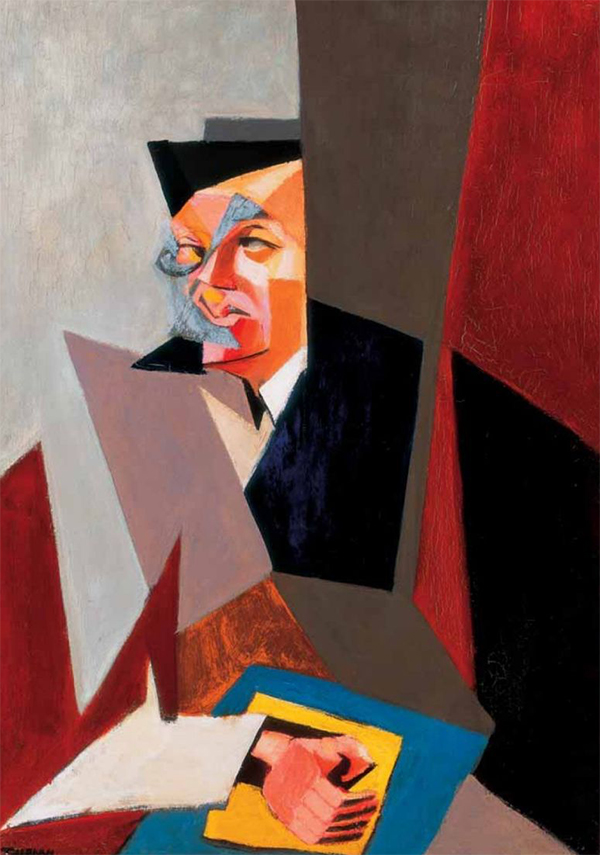
\includegraphics[width=40mm]{stylistic/styles/tihanyi_tzara.jpg}
			}
			\subfloat[Eredmény]{
				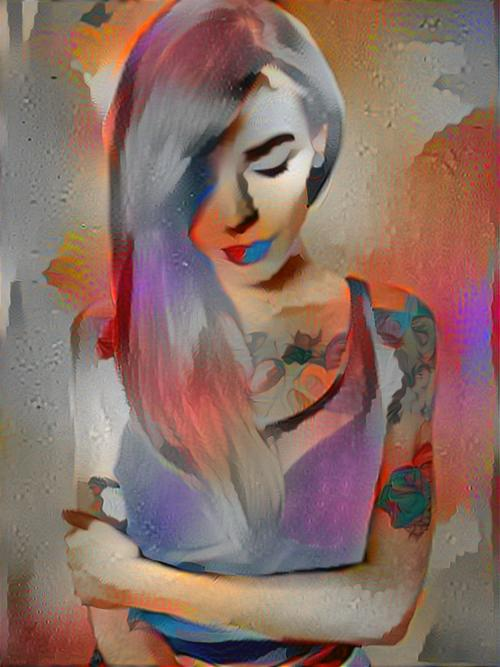
\includegraphics[width=40mm]{stylistic/portre/tihanyi.jpg}
			}
			\caption[]{Tihanyi - Tzara}
			\label{girl_1}
		\end{figure}
	
		\begin{figure}[!htbp]
			\centering
			\subfloat[Stíluskép]{
				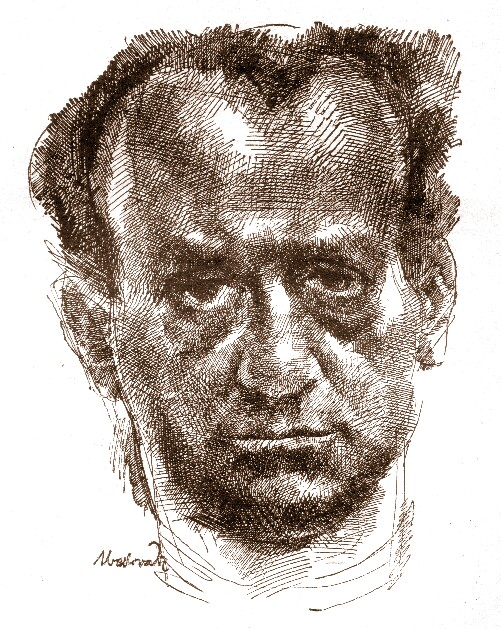
\includegraphics[width=40mm]{stylistic/styles/aba_novak_vilmos_onarckep.jpg}
			}
			\subfloat[Eredmény]{
				\includegraphics[width=40mm]{stylistic/portre/aba.jpg}
			}
			\caption[]{Aba Novák Vilmos - Önarckép}
			\label{girl_2}
		\end{figure}
	
		\begin{figure}[!htbp]
			\centering
			\subfloat[Stíluskép]{
				\includegraphics[width=40mm]{stylistic/styles/reti_alfred.jpg}
			}
			\subfloat[Eredmény]{
				\includegraphics[width=40mm]{stylistic/portre/reti.jpg}
			}
			\caption[]{Réti Alfréd - Kubizmus}
			\label{girl_3}
		\end{figure}
	
		\begin{figure}[!htbp]
			\centering
			\subfloat[Stíluskép]{
				\includegraphics[width=40mm]{stylistic/styles/magyar_nepmesek.jpg}
			}
			\subfloat[Eredmény]{
				\includegraphics[width=40mm]{stylistic/portre/nepmesek.jpg}
			}
			\caption[]{Magyar népmesék}
			\label{girl_4}
		\end{figure}
	
		\begin{figure}[!htbp]
			\begin{center}
				\includegraphics[scale=0.5]{stylistic/original/sapientia.jpg}
				\caption[]{Eredeti kép}
				\label{original_sapientia}
			\end{center}
		\end{figure}
		
		\begin{figure}[!htbp]
			\centering
			\subfloat[Stíluskép]{
				\includegraphics[width=60mm]{stylistic/styles/csontvary_kosztka_tivadar_traui_tajkep_naplemente_idejen.jpg}
			}
			\subfloat[Eredmény]{
				\includegraphics[width=60mm]{stylistic/place/csontvary.jpg}
			}
			\caption[]{Csontváry - Tájkép naplemente idején}
			\label{sapi_1}
		\end{figure}
	
		\begin{figure}[!htbp]
			\centering
			\subfloat[Stíluskép]{
				\includegraphics[width=60mm]{stylistic/styles/munkacsi_mihaly_vihar_a_pusztan.jpg}
			}
			\subfloat[Eredmény]{
				\includegraphics[width=60mm]{stylistic/place/munkacsi.jpg}
			}
			\caption[]{Munkácsi Mihály - Vihar a pusztán}
			\label{sapi_2}
		\end{figure}
	
		\begin{figure}[!htbp]
			\centering
			\subfloat[Stíluskép]{
				\includegraphics[width=60mm]{stylistic/styles/ivanyi_grunwald_bela_parkreszlet_kecskemeten.jpg}
			}
			\subfloat[Eredmény]{
				\includegraphics[width=60mm]{stylistic/place/wald.jpg}
			}
			\caption[]{Grunwald Béla - Parkrészlet Kecskeméten}
			\label{sapi_3}
		\end{figure} 	
	
	\section*{Forráskód}
\end{subappendices}

\end{document}
